% =====================================================================
% Capítulo 1 -- Artigo submetido ao SEPOC (análise cientométrica)
%
% Convenções deste arquivo:
%   \revisor{...}  caixa vermelha  = comentário do revisor (texto original)
%   \sugestao{...}     caixa azul      = sugestão para atender o comentário
%   \pendente{..}  destaque amarelo = item a conferir
%   Citações: padrão ABNT NBR 10520:2023 (autor-data) via abntex2cite:
%   \cite{} = (AUTOR, ano) | \citeonline{} = Autor (ano) no corpo do texto.
% Para gerar a versão limpa, use \mostrarrevisorfalse e \mostrarnotasfalse
% no preâmbulo de thesis.tex.
% =====================================================================

% Este capítulo é baseado no artigo \emph{Aplicações de inteligência artificial na previsão e no mapeamento de inundações: uma análise cientométrica multibase}, de autoria de Daiane Wan-Dall Splitter da Silva e Rodrigo Sant'Ana, submetido ao \emph{18th Seminar on Power Electronics and Control} (SEPOC 2026). O texto foi adaptado ao formato desta dissertação e incorpora as recomendações dos pareceres recebidos.

Este capítulo apresenta o mapeamento cientométrico da literatura sobre inteligência artificial aplicada a inundações. Seu objetivo é caracterizar como essa literatura evoluiu, quais métodos e tarefas a compõem e quais lacunas limitam a transferência dos resultados para aplicações urbanas e costeiras, de modo a orientar a leitura e a revisão da literatura realizadas nesta dissertação.

O texto parte de um artigo de autoria de Daiane Wan-Dall Splitter da Silva e Rodrigo Sant'Ana, submetido ao \emph{18th Seminar on Power Electronics and Control} (SEPOC 2026) com o título ``Aplicações de inteligência artificial na previsão e no mapeamento de inundações: uma análise cientométrica multibase''. Ele foi adaptado ao formato desta dissertação e incorpora as recomendações dos pareceres recebidos, sobretudo quanto à transparência da seleção dos registros, ao escore de priorização e ao mapeamento da estrutura temática.

O capítulo está organizado da seguinte forma: a introdução apresenta o contexto e as perguntas de pesquisa; a metodologia descreve a busca, a deduplicação, a triagem automatizada e o escore de priorização, com sua análise de sensibilidade; os resultados mostram a composição do corpus, a validação externa de cobertura, a evolução temporal, as tecnologias, a estrutura temática, a distribuição geográfica e a síntese dos artigos de maior prioridade; e a discussão, as limitações e a conclusão encerram o texto.

% ---------------------------------------------------------------------
\section{Introdução}
\label{sec:art-introducao}

Inundações resultam da interação entre forçantes meteorológicas e oceânicas, características da bacia, uso do solo, capacidade de drenagem, exposição e vulnerabilidade. Embora a intensificação da precipitação extrema e a elevação do nível do mar ampliem riscos em diversas regiões, principalmente costeiras, tendências observadas de inundação não são espacialmente uniformes e também dependem de urbanização (impermeabilização do solo), intervenções hidráulicas e mudanças na ocupação territorial \cite{ipcc2022,wahl2015}. Em cidades costeiras, a coincidência entre chuva intensa, descarga fluvial e maré elevada pode produzir eventos compostos mais severos do que aqueles gerados por um único processo \cite{wahl2015}.

Modelos hidrológicos, hidráulicos e hidrodinâmicos continuam essenciais para representar mecanismos físicos e testar cenários. Entretanto, sua aplicação operacional pode ser limitada por custo computacional, disponibilidade de dados, calibração local e dificuldade de representar relações não lineares em alta dimensão. Métodos de \textit{machine learning} (ML) e \textit{deep learning} (DL) têm sido utilizados como modelos substitutos, ferramentas de pós-processamento ou componentes híbridos, com aplicações em previsão de chuva/vazão, delimitação de áreas inundadas, classificação de suscetibilidade e sistemas de alerta \cite{mosavi2018,shen2018,kratzert2018,nearing2021}. Resultados recentes demonstram, inclusive, a viabilidade de previsões globais de eventos fluviais extremos em bacias não monitoradas, com modelos treinados em grandes conjuntos de dados \cite{nearing2024}.

O crescimento acelerado do campo dificulta distinguir tendências tecnológicas robustas de efeitos de popularidade, cobertura de base e atraso de citação. Além disso, expressões como ``previsão de inundação'', ``mapeamento de suscetibilidade'', ``detecção de inundação'' e ``avaliação de risco'' representam tarefas científicas diferentes e não devem ser avaliadas pelas mesmas métricas. Análises cientométricas permitem mapear a estrutura de um domínio, desde que a busca, a deduplicação, as unidades de contagem e as limitações de cobertura sejam explicitadas \cite{aria2017}. Recomendações de transparência de revisões estruturadas, como o PRISMA, também são úteis para documentar identificação, triagem e inclusão de registros, ainda que o presente estudo não constitua uma revisão de efeitos de intervenção \cite{page2021}.

Revisões recentes já sintetizaram técnicas de previsão de inundações com inteligência artificial. \citeonline{mosavi2018} revisaram a literatura sobre modelos de aprendizado de máquina para previsão de inundações, e \citeonline{dias2025} analisaram 32 estudos, selecionados de 433 registros conforme o PRISMA, e organizaram uma taxonomia de métodos estatísticos, de \textit{machine learning}, de \textit{deep learning} e híbridos, incluindo sistemas com IoT. Essas revisões respondem à pergunta de quais técnicas existem e como se comparam em um conjunto reduzido de estudos. Este capítulo é complementar e responde a outra pergunta: como é a estrutura da literatura como um todo? Para isso, (i) mapeia de forma cientométrica um corpus de 2.068 artigos, recuperado, na prática, a partir da Lens.org e da Scopus; (ii) documenta de modo reproduzível cada etapa de redução, das exportações brutas ao corpus, com suas falhas de implementação e uma análise de sensibilidade do escore de priorização; (iii) emprega as referências internacionais de \citeonline{dias2025} como referência externa para avaliar a cobertura da busca; e (iv) sintetiza os artigos de maior prioridade segundo a tarefa científica (previsão, detecção, suscetibilidade e risco), o que evidencia que métricas e desenhos de validação não são comparáveis entre tarefas. As lacunas costeiras e compostas, que não foram o foco das revisões anteriores, são discutidas com a ressalva de que parte delas decorre do desenho da busca.

Com base neste contexto, este artigo busca responder a três perguntas: (i) como a produção científica sobre IA e inundações evoluiu temporal e geograficamente? (ii) quais famílias de métodos e tarefas dominam o corpus? e (iii) quais lacunas metodológicas e geográficas limitam a transferência dos resultados para aplicações operacionais, urbanas e costeiras? A contribuição do estudo consiste em integrar múltiplas bases, documentar a redução do corpus e interpretar os resultados à luz das diferenças entre previsão temporal, detecção, suscetibilidade e risco.

% ---------------------------------------------------------------------
\section{Metodologia}
\label{sec:art-metodologia}

\subsection{Desenho do estudo}

Foi realizada uma análise cientométrica descritiva, complementada por síntese narrativa dos artigos de maior prioridade. O fluxo de identificação e seleção foi apresentado segundo o formato de relato do PRISMA \cite{page2021}, o que organiza a documentação das etapas, mas não implica uma revisão sistemática com triagem manual por pares: a seleção foi automatizada e é descrita na Seção~\ref{sec:art-triagem}. Os indicadores bibliométricos seguiram práticas de harmonização e mapeamento científico descritas por \citeonline{aria2017}.

\subsection{Estratégia de busca e elegibilidade}

As buscas foram conduzidas nas bases Lens.org, Scopus, IEEE Xplore e SciELO, abrangendo publicações de 1992 a 2026, sendo 2026 um ano parcial. A expressão original, adaptada apenas à sintaxe de cada plataforma, foi:

\begin{quote}\small
(``flood prediction'' OR ``flood forecasting'' OR ``flood risk'' OR ``flood modeling'' OR ``urban flooding'' OR ``inundation'') AND (``machine learning'' OR ``deep learning'' OR ``artificial intelligence'').
\end{quote}

Os critérios de elegibilidade foram implementados como regras de correspondência de termos, por busca de trechos de texto sem distinção de caixa, sobre título, resumo e palavras-chave. Foram retidos os registros que continham, simultaneamente: (i) ao menos um de 18 termos de inundação ou previsão (por exemplo, \textit{flood prediction}, \textit{flood forecasting}, \textit{flood risk}, \textit{flooding}, ``inundação urbana''); (ii) ao menos um de 20 termos de IA/ML (por exemplo, \textit{machine learning}, \textit{deep learning}, LSTM, \textit{random forest}, \textit{ensemble}); e (iii) ao menos um de 40 termos de dados hidrológicos ou geoespaciais no resumo ou nas palavras-chave (por exemplo, \textit{rainfall}, \textit{river}, \textit{satellite}, \textit{remote sensing}). Foram excluídos os registros cujo título ou resumo continha algum de 15 termos de exclusão (por exemplo, \textit{flood insurance}, \textit{flood myth}, \textit{buffer overflow}, \textit{dam}, \textit{levee}). Como o casamento é por trecho de texto, termos curtos casam dentro de outras palavras (\textit{dam} em \textit{damage}); esse efeito é quantificado na Seção~\ref{sec:art-sensibilidade}. As listas completas e o código estão no material suplementar de replicação.

A expressão de busca não incluiu explicitamente termos como \textit{coastal flooding}, \textit{storm surge}, \textit{compound flooding}, \textit{pluvial flooding} e \textit{flash-flood nowcasting}. Essa decisão afeta a sensibilidade da busca para estudos costeiros e compostos e é tratada como limitação, não como evidência de ausência da literatura.

\subsection{Deduplicação e fluxo de seleção}

Foram identificados 16.845 registros, correspondentes à soma de oito arquivos de exportação (Lens em inglês e em português; Scopus, em três arquivos, dois deles com sobreposição de conteúdo por serem exportações com e sem filtro da plataforma; IEEE Xplore, com 612 registros; e SciELO em inglês e em português). Esse total, portanto, é uma contagem de registros nos arquivos e não de documentos distintos. A deduplicação ocorreu em duas etapas. Na primeira, por DOI, restaram 12.470 registros: foram removidos 4.375, dos quais 3.836 eram duplicatas e 539 eram registros sem DOI, que o procedimento descarta por manter apenas linhas com DOI. Na segunda, por título normalizado quanto à caixa, foram removidos 923, restando 11.547 registros únicos. A reexecução do código reproduziu esses totais (removidos: 5.298), mas não a divisão entre etapas registrada originalmente (4.233 por DOI e 1.065 por título).

Duas limitações de implementação afetaram a composição do corpus. Primeiro, o mapeamento de colunas não reconheceu os campos de título do IEEE Xplore (``Document Title'') nem os campos de ano, resumo, palavras-chave e DOI da SciELO em inglês; os registros ficaram sem título (valor ausente) e colapsaram na deduplicação por título, e os sem DOI foram descartados, de modo que, na prática, o corpus provém da Lens e da Scopus. Segundo, a coluna de palavras-chave da Scopus não foi reconhecida, e a elegibilidade desses registros apoiou-se em título e resumo. Ambos os pontos são tratados como limitações (Seção~\ref{sec:art-limitacoes}).

\subsection{Triagem temática e validação do procedimento}
\label{sec:art-triagem}

A triagem temática foi inteiramente automatizada. Em vez de um revisor decidir, registro a registro, se um artigo era elegível, a decisão foi tomada por regras escritas em código: o programa procura, no título, no resumo e nas palavras-chave de cada registro, listas de termos definidas previamente. Essa escolha tem uma vantagem e um custo. A vantagem é a reprodutibilidade: a mesma entrada produz sempre o mesmo resultado, sem depender de julgamento individual. O custo é a rigidez: a regra só reconhece os termos listados, de modo que sinônimos não previstos são perdidos e termos polissêmicos, ou contidos em outras palavras, podem ser aceitos ou rejeitados indevidamente.

A regra tem duas partes, aplicadas em sequência aos 11.547 registros únicos (Tabela~\ref{tab:regra}). Primeiro vem a inclusão: o registro precisa conter pelo menos um termo de cada um dos três grupos. Depois vem a exclusão: entre os que passaram, são removidos os que contêm algum termo de exclusão. As listas completas estão no material de replicação.

\begin{table}[!htb]
\centering
\caption{Regras da triagem temática automatizada.}
\label{tab:regra}
{\small
\renewcommand{\arraystretch}{1.2}
\begin{tabular}{@{}p{1.9cm}p{3.2cm}p{5.4cm}p{2.6cm}@{}}
\toprule
\textbf{Etapa} & \textbf{Condição} & \textbf{Termos (exemplos)} & \textbf{Campos}\\
\midrule
Inclusão 1 & Inundação ou previsão & 18 termos: \textit{flood prediction}, \textit{flood forecasting}, \textit{flood risk}, \textit{flooding}, ``inundação urbana'' & título, resumo e palavras-chave\\
Inclusão 2 & IA ou aprendizado de máquina & 20 termos: \textit{machine learning}, \textit{deep learning}, LSTM, \textit{random forest}, \textit{ensemble} & título, resumo e palavras-chave\\
Inclusão 3 & Dados hidrológicos ou geoespaciais & 40 termos: \textit{rainfall}, \textit{river}, \textit{satellite}, \textit{remote sensing} & resumo e palavras-chave\\
Exclusão & Fora do escopo & 15 termos: \textit{flood insurance}, \textit{flood myth}, \textit{buffer overflow}, \textit{dam}, \textit{levee} & título e resumo\\
\bottomrule
\end{tabular}}\\[2mm]
{\small Fonte: Elaborado pela autora.}
\end{table}

Dos 11.547 registros únicos, 2.068 foram mantidos e 9.479 foram excluídos. Esses 9.479 têm duas origens: 8.853 não satisfaziam ao menos um dos três grupos de inclusão (fora do escopo temático), e 626 satisfaziam os três, mas continham um termo de exclusão. Entre esses 626, 498 foram excluídos apenas porque um termo curto de exclusão (\textit{dam}) casou dentro de outra palavra, uma falha de implementação discutida na Seção~\ref{sec:art-sensibilidade}. O fluxo completo é apresentado na Figura~\ref{fig:fluxo}.

Um exemplo mostra a regra em funcionamento. A revisão de \citeonline{mosavi2018} contém termos dos três grupos de inclusão e, por isso, chegou à etapa de exclusão; seu resumo, porém, menciona \textit{property damage}, e o termo de exclusão \textit{dam} casa dentro de \textit{damage}. O registro foi removido, embora seja pertinente. É esse tipo de erro que a análise da Seção~\ref{sec:art-sensibilidade} quantifica.

Como a decisão de elegibilidade não envolveu revisores, não há número de avaliadores, desacordos a resolver nem estatística de concordância, como o $\kappa$ de Cohen, a reportar: a decisão é plenamente determinada pelas listas de termos. Por não ter passado por revisão humana, a validade da regra foi examinada por três verificações: (i) a reexecução do código original sobre os arquivos brutos, que reproduziu exatamente as contagens do fluxo (16.845, 11.547 e 2.068) e dos estratos e permitiu identificar suas falhas; (ii) a análise de sensibilidade do escore (Seção~\ref{sec:art-sensibilidade}); e (iii) a validação externa de cobertura frente às referências de \citeonline{dias2025} (Seção~\ref{sec:art-validacao}). Adicionalmente, a elegibilidade dos 13 artigos do Núcleo A foi conferida manualmente pela autora contra quatro critérios explícitos (inundação, IA/ML, previsão ou mapeamento e uso de dados hidrológicos ou geoespaciais). 
%\pendente{concluir a conferência dos itens sinalizados: \#2 (sem menção a inundação nos metadados), \#1, \#3 e \#12 (escopo), \#7 (resumo ausente na base)}.

\pendente{O código que implementa a triagem está disponível no repositório de replicação \url{https://github.com/DWan-Dall/dashboard-cientometria} (versão 0.2.1, etiqueta \texttt{v0.2.1-dissertacao}, \textit{commit} \texttt{adfa0e1})}

\begin{figure}[!htb]
\centering
\caption{Fluxo de identificação, deduplicação, triagem automatizada e estratificação do corpus, no formato de relato do PRISMA. A triagem foi automatizada, sem avaliação manual por revisores. O total de 16.845 soma as exportações e inclui duas exportações sobrepostas da Scopus. Todos os valores foram reproduzidos pela reexecução do código sobre os arquivos brutos.}
\label{fig:fluxo}
\begin{tikzpicture}[
  font=\footnotesize,
  main/.style={draw, rounded corners=2pt, align=center, inner sep=3pt, minimum height=10mm, text width=5.0cm},
  side/.style={draw, dashed, rounded corners=2pt, align=left, inner sep=3pt, text width=4.9cm, fill=black!5},
  fase/.style={draw=none, fill=black!12, rounded corners=2pt, align=center, inner sep=3pt, text width=1.9cm, font=\scriptsize\bfseries},
  seta/.style={-{Latex[length=2mm]}, thick},
  node distance=11mm]
  % coluna principal
  \node[main] (m1) {\textbf{Registros nas exportações}\\ \textit{n} = 16.845\\ Lens (EN, PT); Scopus (3 arq.);\\ IEEE Xplore (612);\\ SciELO (EN, PT)};
  \node[main, below=of m1] (m2) {\textbf{Após deduplicação por DOI}\\ \textit{n} = 12.470};
  \node[main, below=of m2] (m3) {\textbf{Registros únicos}\\ (título normalizado)\\ \textit{n} = 11.547};
  \node[main, below=of m3] (m4) {\textbf{Satisfazem os três grupos de inclusão}\\ \textit{n} = 2.694};
  \node[main, below=of m4] (m5) {\textbf{Corpus analisado}\\ \textit{n} = 2.068};
  \node[main, below=of m5] (m6) {\textbf{Estratificação pelo escore (0--100)}\\ Núcleo A ($\geq$70): 13\\ Núcleo B (50--70): 494\\ Periférico (30--50): 1.508\\ Descarte ($<$30): 53};
  % pontos nas setas, para as caixas laterais
  \path (m1) -- (m2) coordinate[pos=.5] (x12);
  \path (m2) -- (m3) coordinate[pos=.5] (x23);
  \path (m3) -- (m4) coordinate[pos=.5] (x34);
  \path (m4) -- (m5) coordinate[pos=.5] (x45);
  \node[side, anchor=west] (s2) at ([xshift=6mm]m1.east |- x12) {\textbf{Removidos: 4.375}\\ 3.836 duplicatas de DOI\\ 539 sem DOI (descartados)};
  \node[side, anchor=west] (s3) at ([xshift=6mm]m1.east |- x23) {\textbf{Removidos: 923}\\ duplicatas por título normalizado};
  \node[side, anchor=west] (s4) at ([xshift=6mm]m1.east |- x34) {\textbf{Excluídos: 8.853}\\ não atendem a pelo menos um grupo: (1) inundação ou previsão; (2) IA/ML; (3) dados hidrológicos ou geoespaciais};
  \node[side, anchor=west] (s5) at ([xshift=6mm]m1.east |- x45) {\textbf{Excluídos: 626}\\ termo de exclusão no título ou resumo (498 apenas por \textit{dam} dentro de \textit{damage})};
  % fases
  \node[fase, anchor=east] at ([xshift=-3mm]m1.west) {Identificação};
  \path (m2) -- (m3) coordinate[pos=.5] (c23);
  \node[fase, anchor=east] at ([xshift=-3mm]m1.west |- c23) {Deduplicação};
  \path (m4) -- (m5) coordinate[pos=.5] (c45);
  \node[fase, anchor=east] at ([xshift=-3mm]m1.west |- c45) {Triagem temática};
  \node[fase, anchor=east] at ([xshift=-3mm]m1.west |- m6) {Estratificação};
  % setas
  \foreach \a/\b in {m1/m2, m2/m3, m3/m4, m4/m5, m5/m6} \draw[seta] (\a) -- (\b);
  \foreach \x/\s in {x12/s2, x23/s3, x34/s4, x45/s5} \draw[seta] (\x) -- (\s.west);
\end{tikzpicture}\\[2mm]
{\small Fonte: Elaborado pela autora.}
\end{figure}

\subsection{Escore de priorização}
\label{sec:art-escore}

Depois da triagem, restam 2.068 artigos, número grande demais para leitura integral. O escore de priorização serve para ordenar esse conjunto e decidir por onde começar a leitura. Ele não mede a qualidade científica de um artigo: combina quatro sinais simples e verificáveis, cada um transformado em um número entre 0 e 1, e os soma com pesos diferentes (Tabela~\ref{tab:escore}).

\begin{table}[!htb]
\centering
\caption{Componentes do escore de priorização.}
\label{tab:escore}
{\small
\renewcommand{\arraystretch}{1.2}
\begin{tabular}{@{}p{2.4cm}p{1cm}p{3.1cm}p{6.3cm}@{}}
\toprule
\textbf{Componente} & \textbf{Peso} & \textbf{Pergunta que responde} & \textbf{Como é calculado}\\
\midrule
$C^{*}$ Citações & 0,35 & O artigo é muito citado? & Citações na base, reescaladas de 0 a 1 entre o mínimo (0) e o máximo (555) do corpus.\\
$R^{*}$ Recência & 0,20 & É recente? & $(\text{ano}-1992)/(2026-1992)$; os nove registros sem ano recebem 0.\\
$T^{*}$ Aderência temática & 0,30 & Trata de inundação e de IA já no título? & 1,0 se o título contém termo de inundação ou previsão e termo de IA/ML; 0,7 se essa coocorrência só aparece no conjunto de título, resumo e palavras-chave; 0,4 nos demais casos.\\
$A^{*}$ Dados, método e resultado & 0,15 & Descreve dados, método e resultado? & Média de quatro indicadores, $I$, $M$, $O$ e $C$, detalhados abaixo.\\
\bottomrule
\end{tabular}}\\[2mm]
{\small Fonte: Elaborado pela autora.}
\end{table}

A estrutura do escore, os pesos, os cortes e as listas de termos foram propostos com apoio do Perplexity AI e adotados pela autora, sem calibração empírica própria; por isso, sua influência sobre o resultado é examinada na Seção~\ref{sec:art-sensibilidade}. Para cada artigo $i$, o escore é
%
\begin{equation}
S_i = 0{,}35\,C_i^{*} + 0{,}20\,R_i^{*} + 0{,}30\,T_i^{*} + 0{,}15\,A_i^{*}.
\label{eq:escore}
\end{equation}

Dois componentes dependem de listas de termos e merecem explicação. O $T^{*}$ distingue os artigos que anunciam o tema no título dos que apenas o mencionam no resumo; nenhum registro recebeu 0,4, porque o filtro já exige a coocorrência, e 514 registros tiveram $T^{*}=1{,}0$ e 1.554 tiveram 0,7. O $A^{*}$ é a média de quatro indicadores, cada um valendo 1 se uma condição é verificada e 0,5 caso contrário (exceto o primeiro, que vale 0 ou 1):
%
\begin{itemize}
  \item $I$ (dados): vale 1 se o resumo ou as palavras-chave contêm termo de dados hidrológicos ou geoespaciais. Vale 1 para todo o corpus, pois o filtro já exige esse termo;
  \item $M$ (método): vale 1 se título ou resumo contêm termo de método. A lista inclui algoritmos, como LSTM, CNN e \textit{random forest}, e termos genéricos, como \textit{machine learning} e \textit{neural network}; cerca de metade dos registros recebeu 1 apenas por termo genérico;
  \item $O$ (objetivo): vale 1 se título ou resumo mencionam previsão, alerta ou mapeamento;
  \item $C$ (contexto): vale 1 se o resumo ou as palavras-chave mencionam contexto urbano, costeiro, de bacia ou de rio.
\end{itemize}
%
Como $I$ é sempre 1 e os demais valem no mínimo 0,5, $A^{*}$ variou de 0,625 a 1.

\paragraph{Como ler o resultado.} O valor bruto de $S_i$ é reescalado de 0 a 100 pelo mínimo e pelo máximo do corpus. O valor 100 corresponde, assim, ao artigo de maior escore dentro deste corpus, e não a um padrão absoluto de qualidade. Os cortes são relativos ao mesmo corpus: Núcleo A com escore $\geq 70$; Núcleo B de 50 a 70; Periférico de 30 a 50; e Descarte abaixo de 30.

\paragraph{Exemplo ilustrativo.} Considere um artigo hipotético de 2019, com 111 citações, cujo título contém termos de inundação e de IA, e cujo resumo contém termos de dados, de método e de previsão, mas nenhum de contexto. Então $C^{*}=111/555=0{,}20$; $R^{*}=(2019-1992)/34\approx 0{,}79$; $T^{*}=1{,}0$; e $A^{*}=(1+1+1+0{,}5)/4=0{,}875$. O escore bruto é $0{,}35\cdot 0{,}20+0{,}20\cdot 0{,}79+0{,}30\cdot 1{,}0+0{,}15\cdot 0{,}875\approx 0{,}66$, valor que depois é reescalado de 0 a 100. O exemplo mostra por que artigos antigos e muito citados são favorecidos pelo $C^{*}$, e por que um artigo recente com título aderente também pode ter boa posição.

Quanto ao procedimento de codificação e à concordância entre avaliadores, nenhum componente do escore depende de julgamento humano: $T^{*}$ e $A^{*}$ são calculados por presença de termos e $C^{*}$ e $R^{*}$ por aritmética sobre os metadados. Não há, portanto, codificadores nem concordância a medir. A robustez da classificação resultante é testada na seção seguinte.

\subsection{Análise de sensibilidade do escore}
\label{sec:art-sensibilidade}

Como os pesos foram propostos com apoio de ferramenta de IA e adotados sem calibração empírica própria, testou-se a estabilidade do Núcleo A frente a variações dos pesos, recalculando o escore sobre os mesmos 2.068 artigos (componentes $C^*$, $R^*$, $T^*$ e $A^*$ fixos). Em 10.000 simulações, cada peso foi multiplicado por um fator independente entre 0,85 e 1,15, sem renormalização explícita, pois o ranking é invariante à escala comum dos pesos e o escore final é reescalado de 0 a 100. Em todas as simulações, ao menos 11 dos 13 artigos originais permaneceram entre os 13 primeiros do ranking (média de 12,2; os 13 permaneceram em 24,8\% das simulações). A variação de um único peso em $\pm 15\%$ manteve 12 ou 13 artigos, e pesos iguais para os quatro componentes mantiveram 11. A classificação é, portanto, robusta a perturbações moderadas, mas não a mudanças grandes: sorteando pesos de uma distribuição de Dirichlet com concentração 5, a média de retenção caiu para 9,1 artigos e apenas 35,6\% das simulações mantiveram 11 ou mais. Além disso, o corte fixo em 70 pontos é frágil: quatro artigos têm escore entre 70,2 e 71,1, logo acima do corte, e o tamanho do Núcleo A variou de 7 a 45 artigos nas simulações de $\pm 15\%$. Por essa razão, o ranking relativo é mais defensável do que o corte absoluto.

A estabilidade foi testada também frente à composição do corpus. A exclusão por trecho de texto remove artigos pertinentes: dos 2.694 registros que satisfaziam os demais critérios, 626 foram excluídos e 498 deles apenas porque um termo curto de exclusão (\textit{dam}) aparecia dentro de outra palavra (\textit{damage}), entre eles \citeonline{mosavi2018}, revisão de previsão de inundações com ML e 1.008 citações na Lens (1.203 na Scopus; a cópia mantida na deduplicação é a da Lens). Refazendo o fluxo com a exclusão restrita a palavras inteiras (corpus de 2.566 registros, demais regras idênticas), o artigo de Mosavi et al. entra no corpus e o máximo de citações passa de 555 para 1.008; como $C^{*}$ é normalizado pelo máximo, os escores dos demais diminuem, e apenas esse artigo atinge 70 pontos. Os 13 artigos originais passam a ter de 48,7 a 62,6 pontos (12 no Núcleo B e 1 no Periférico). Em posição no ranking, porém, 12 dos 13 permanecem entre as 25 primeiras de 2.566 (posições 5 a 25), e um (o estudo de detecção e suscetibilidade com Sentinel-1) cai para a 401.ª. O rótulo ``Núcleo A'' é, portanto, uma propriedade do corpus e do artigo mais citado, e não uma classe estável; o ranking é a evidência mais defensável de prioridade, e os 13 artigos devem ser entendidos como o topo do ranking do procedimento original, e não como um conjunto invariante.

\subsection{Indicadores e mapeamento científico estrutural}

Este estudo é descritivo: seu objetivo é mapear o que foi publicado, e não explicar as relações entre os autores ou reconstruir a história intelectual do campo. Por isso, a maior parte dos indicadores é descritiva, como o número anual de artigos, a distribuição de citações por ano, a frequência de categorias tecnológicas e os países de afiliação. Além desses indicadores, foram feitas análises de mapeamento científico estrutural, e outras foram calculadas pela ferramenta, mas não interpretadas (Tabela~\ref{tab:mapeamento}).

\begin{table}[!htb]
\centering
\caption{Análises de mapeamento científico: situação neste estudo.}
\label{tab:mapeamento}
{\small
\renewcommand{\arraystretch}{1.2}
\begin{tabular}{@{}p{5.2cm}p{3.3cm}p{4.3cm}@{}}
\toprule
\textbf{Análise} & \textbf{Situação} & \textbf{Onde aparece}\\
\midrule
Indicadores descritivos (produção, citações, países) & Realizada e interpretada & Seção~\ref{sec:art-resultados}\\
Coocorrência dos 31 termos tecnológicos mais frequentes (203 pares) & Realizada e interpretada & Esta seção\\
Coocorrência de 614 termos (7.864 pares), agrupamentos de Louvain e mapa temático & Realizada e interpretada & Seção~\ref{sec:art-estrutura}\\
Evolução anual das categorias de métodos & Realizada e interpretada & Seção~\ref{sec:art-estrutura}\\
Cocitação, acoplamento bibliográfico e coautoria & Calculadas, não interpretadas & Agenda de pesquisa\\
Evolução temática por fatiamento do período & Não realizada & Agenda de pesquisa\\
\bottomrule
\end{tabular}}\\[2mm]
{\small Fonte: Elaborado pela autora.}
\end{table}

As frequências de palavras-chave foram complementadas por uma rede de coocorrência dos 31 termos tecnológicos mais frequentes, ou seja, termos que aparecem juntos nos mesmos artigos. A rede tem 203 pares e resultou em um único componente conexo, sem separação temática interna evidente (Figura~\ref{fig:rede31}). Para uma visão mais ampla, a estrutura temática foi explorada por uma rede de 614 termos e 7.864 pares, com agrupamentos pelo método de Louvain (semente 123), posicionados em um mapa temático por centralidade e densidade; a evolução tecnológica foi descrita pela frequência anual de categorias de métodos (Seção~\ref{sec:art-estrutura}).

\begin{figure}[!htb]
\centering
\caption{Rede de coocorrência dos 31 termos tecnológicos mais frequentes. O tamanho de cada círculo é proporcional à frequência do termo e a espessura da linha, ao número de artigos em que os dois termos aparecem juntos.}
\label{fig:rede31}
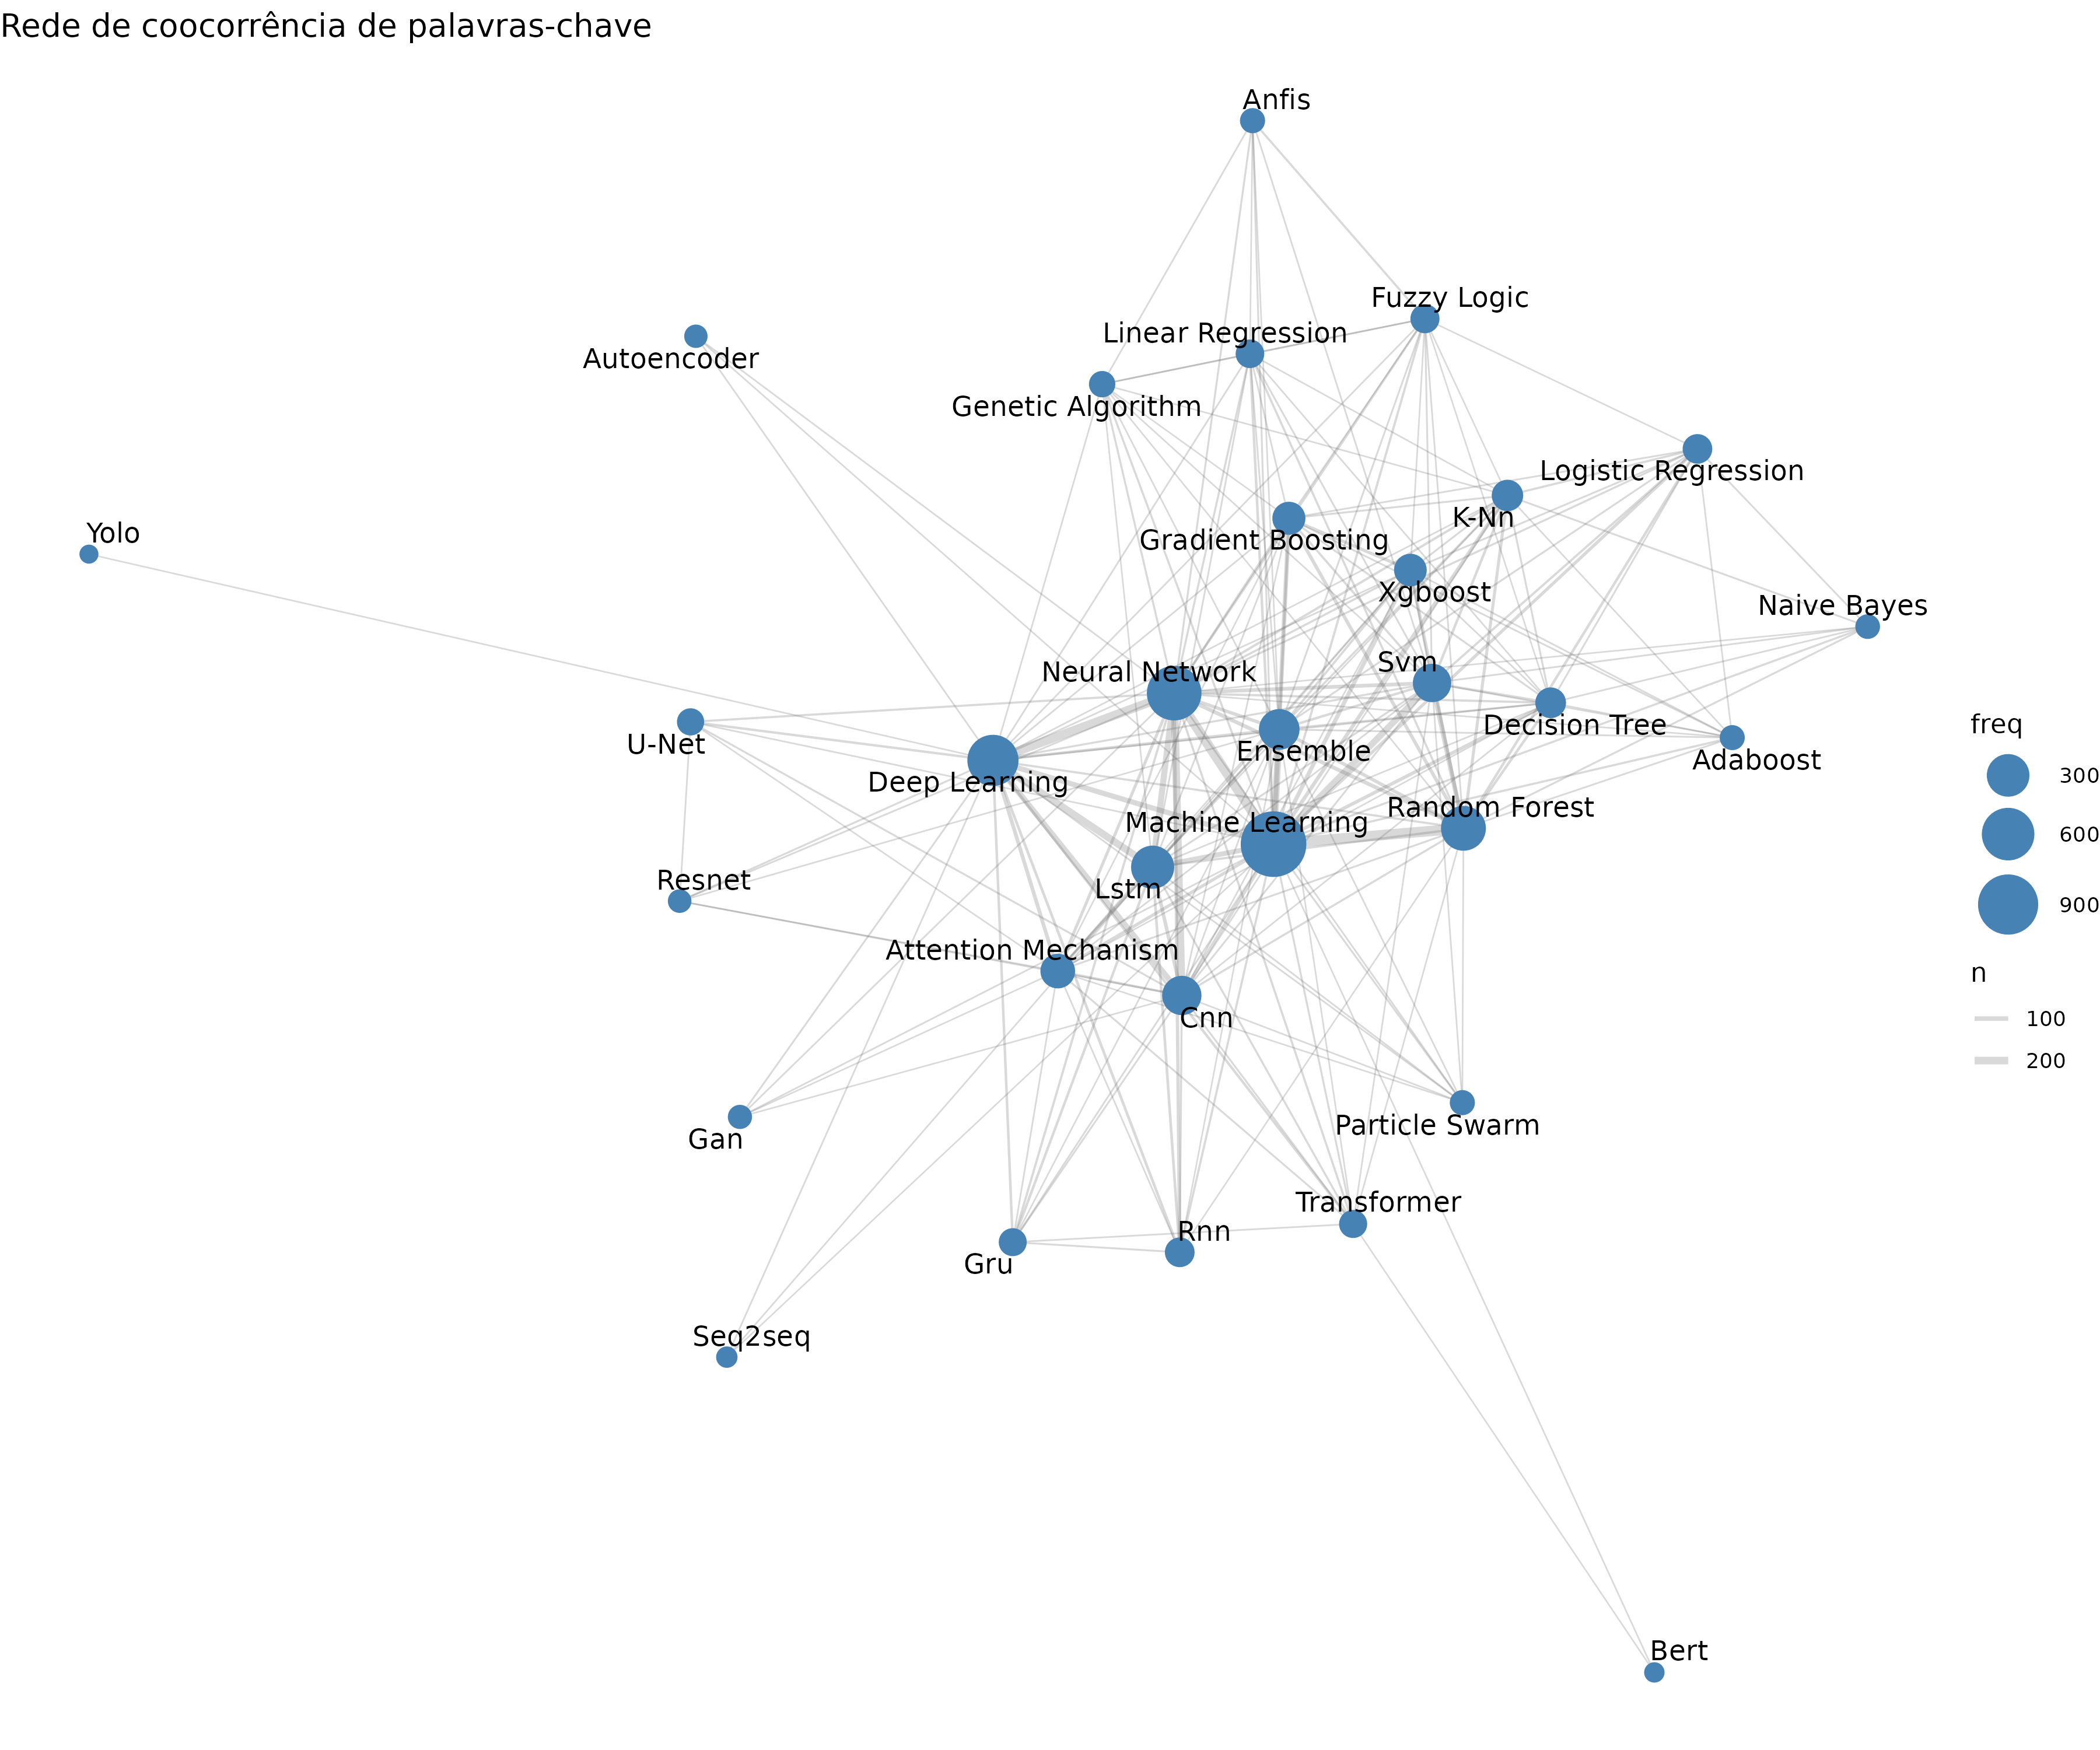
\includegraphics[width=0.85\textwidth]{imagens/sepoc-fig-rede-31-termos.png}\\[2mm]
{\small Fonte: Elaborado pela autora.}
\end{figure}

Cocitação, acoplamento bibliográfico e coautoria foram calculados pela ferramenta, mas não são interpretados neste estudo, porque os dados de entrada ainda não são comparáveis entre as bases. Nas referências, a Lens fornece identificadores e a Scopus, texto livre (dos 33.198 itens distintos, 29.490 são identificadores da Lens e 3.708 são texto livre da Scopus), de modo que o acoplamento bibliográfico praticamente não liga as duas bases (351 de 72.231 arestas). Na coautoria, a ferramenta não leu o campo de autores da Lens: só 463 dos 2.068 documentos têm autores, todos da Scopus, e os formatos de nome diferem entre as bases, o que duplicaria a mesma pessoa em dois nós. A evolução temática por fatiamento do período não foi realizada. Essas análises compõem a agenda de continuidade (Seção~\ref{sec:art-discussao}).

Assim, a contribuição deste estudo é de natureza descritiva e metodológica: um panorama quantitativo da literatura sobre inteligência artificial aplicada a inundações, um protocolo de seleção e priorização explícito e reprodutível, com suas falhas documentadas, e a identificação de lacunas, em especial a escassez de estudos costeiros. Ele não pretende propor um novo método cientométrico nem estabelecer as redes intelectuais do campo.

Contagens geográficas representam afiliações presentes nos metadados, não necessariamente o local empírico do estudo. As citações correspondem ao estado das bases na data de extração e estão sujeitas a diferenças de cobertura e atraso de acumulação.

% ---------------------------------------------------------------------
\section{Resultados}
\label{sec:art-resultados}

\subsection{Composição do corpus}

A deduplicação reteve 68,5\% dos 16.845 registros inicialmente identificados. Após a filtragem temática automatizada, 2.068 documentos permaneceram para a análise, equivalentes a 17,9\% dos registros únicos. O Núcleo A correspondeu a 0,63\% do corpus analisado, enquanto os Núcleos A e B, em conjunto, reuniram 507 documentos (24,5\%). Esses percentuais descrevem a intensidade da triagem, não sua validade, examinada na Seção~\ref{sec:art-validacao}.

\subsection{Validação externa de cobertura}
\label{sec:art-validacao}

Como não houve avaliação manual da triagem, a cobertura do procedimento foi testada contra um conjunto independente: as 22 referências internacionais de \citeonline{dias2025}, selecionadas por uma revisão sistemática segundo o PRISMA (as 10 demais referências são dissertações, relatórios e literatura cinzenta nacional, fora do alcance das bases consultadas). Os títulos foram localizados por similaridade textual ($\geq 0{,}90$) nos 16.845 registros brutos e acompanhados ao longo do fluxo. Dez das 22 (45\%) foram localizadas; oito passaram no filtro temático, três delas foram barradas por termos de exclusão (entre as quais \citeonline{mosavi2018}, por \textit{dam} em \textit{damage}) e cinco chegaram ao corpus de 2.068 artigos, sendo quatro no Núcleo B e uma no estrato Periférico; nenhuma integrou o Núcleo A. Doze não foram localizadas; parte delas pode estar nos arquivos do IEEE Xplore, cujo campo de título não foi lido pelo código, o que impede a comparação por título. Assim, as perdas ocorrem em dois pontos: na busca e na recuperação (doze referências) e no filtro, por limitação de implementação (duas fora do filtro e três por termo de exclusão).

Esse resultado indica que o escore prioriza de forma consistente o que o corpus contém, mas que a cobertura da literatura central é parcial, sobretudo por limitações da estratégia de busca. Ele não invalida o mapeamento, mas condiciona sua interpretação: os 13 artigos do Núcleo A são os de maior prioridade \textit{dentro do corpus recuperado}, e não necessariamente os mais relevantes da literatura.

\subsection{Evolução temporal e padrão de citações}

A produção aumentou acentuadamente a partir de 2018. O ano de 2025 reuniu 578 artigos, ou 27,9\% do corpus elegível, e o intervalo 2019--2025 concentrou aproximadamente 93,3\% das publicações. O valor de 2026 não deve ser comparado aos anos completos devido à extração parcial e ao atraso de indexação (Figura~\ref{fig:producao}).

A distribuição de citações foi fortemente assimétrica, com poucos artigos concentrando uma grande parcela do impacto observado (Figura~\ref{fig:citacoes}). Os totais mais elevados nas coortes intermediárias refletem simultaneamente a visibilidade e o tempo de exposição. Consequentemente, as citações brutas favorecem documentos mais antigos, enquanto os anos recentes ainda não completaram sua janela de acumulação.

\begin{figure}[!htb]
\centering
\caption{Dinâmica temporal do corpus selecionado. Em (a), 2026 representa um ano parcial. Em (b), as citações são apresentadas em escala bruta e refletem a data de extração, a cobertura das bases e o tempo de acumulação.}
\label{fig:dinamica}
\begin{subfigure}[t]{0.49\textwidth}
  \centering
  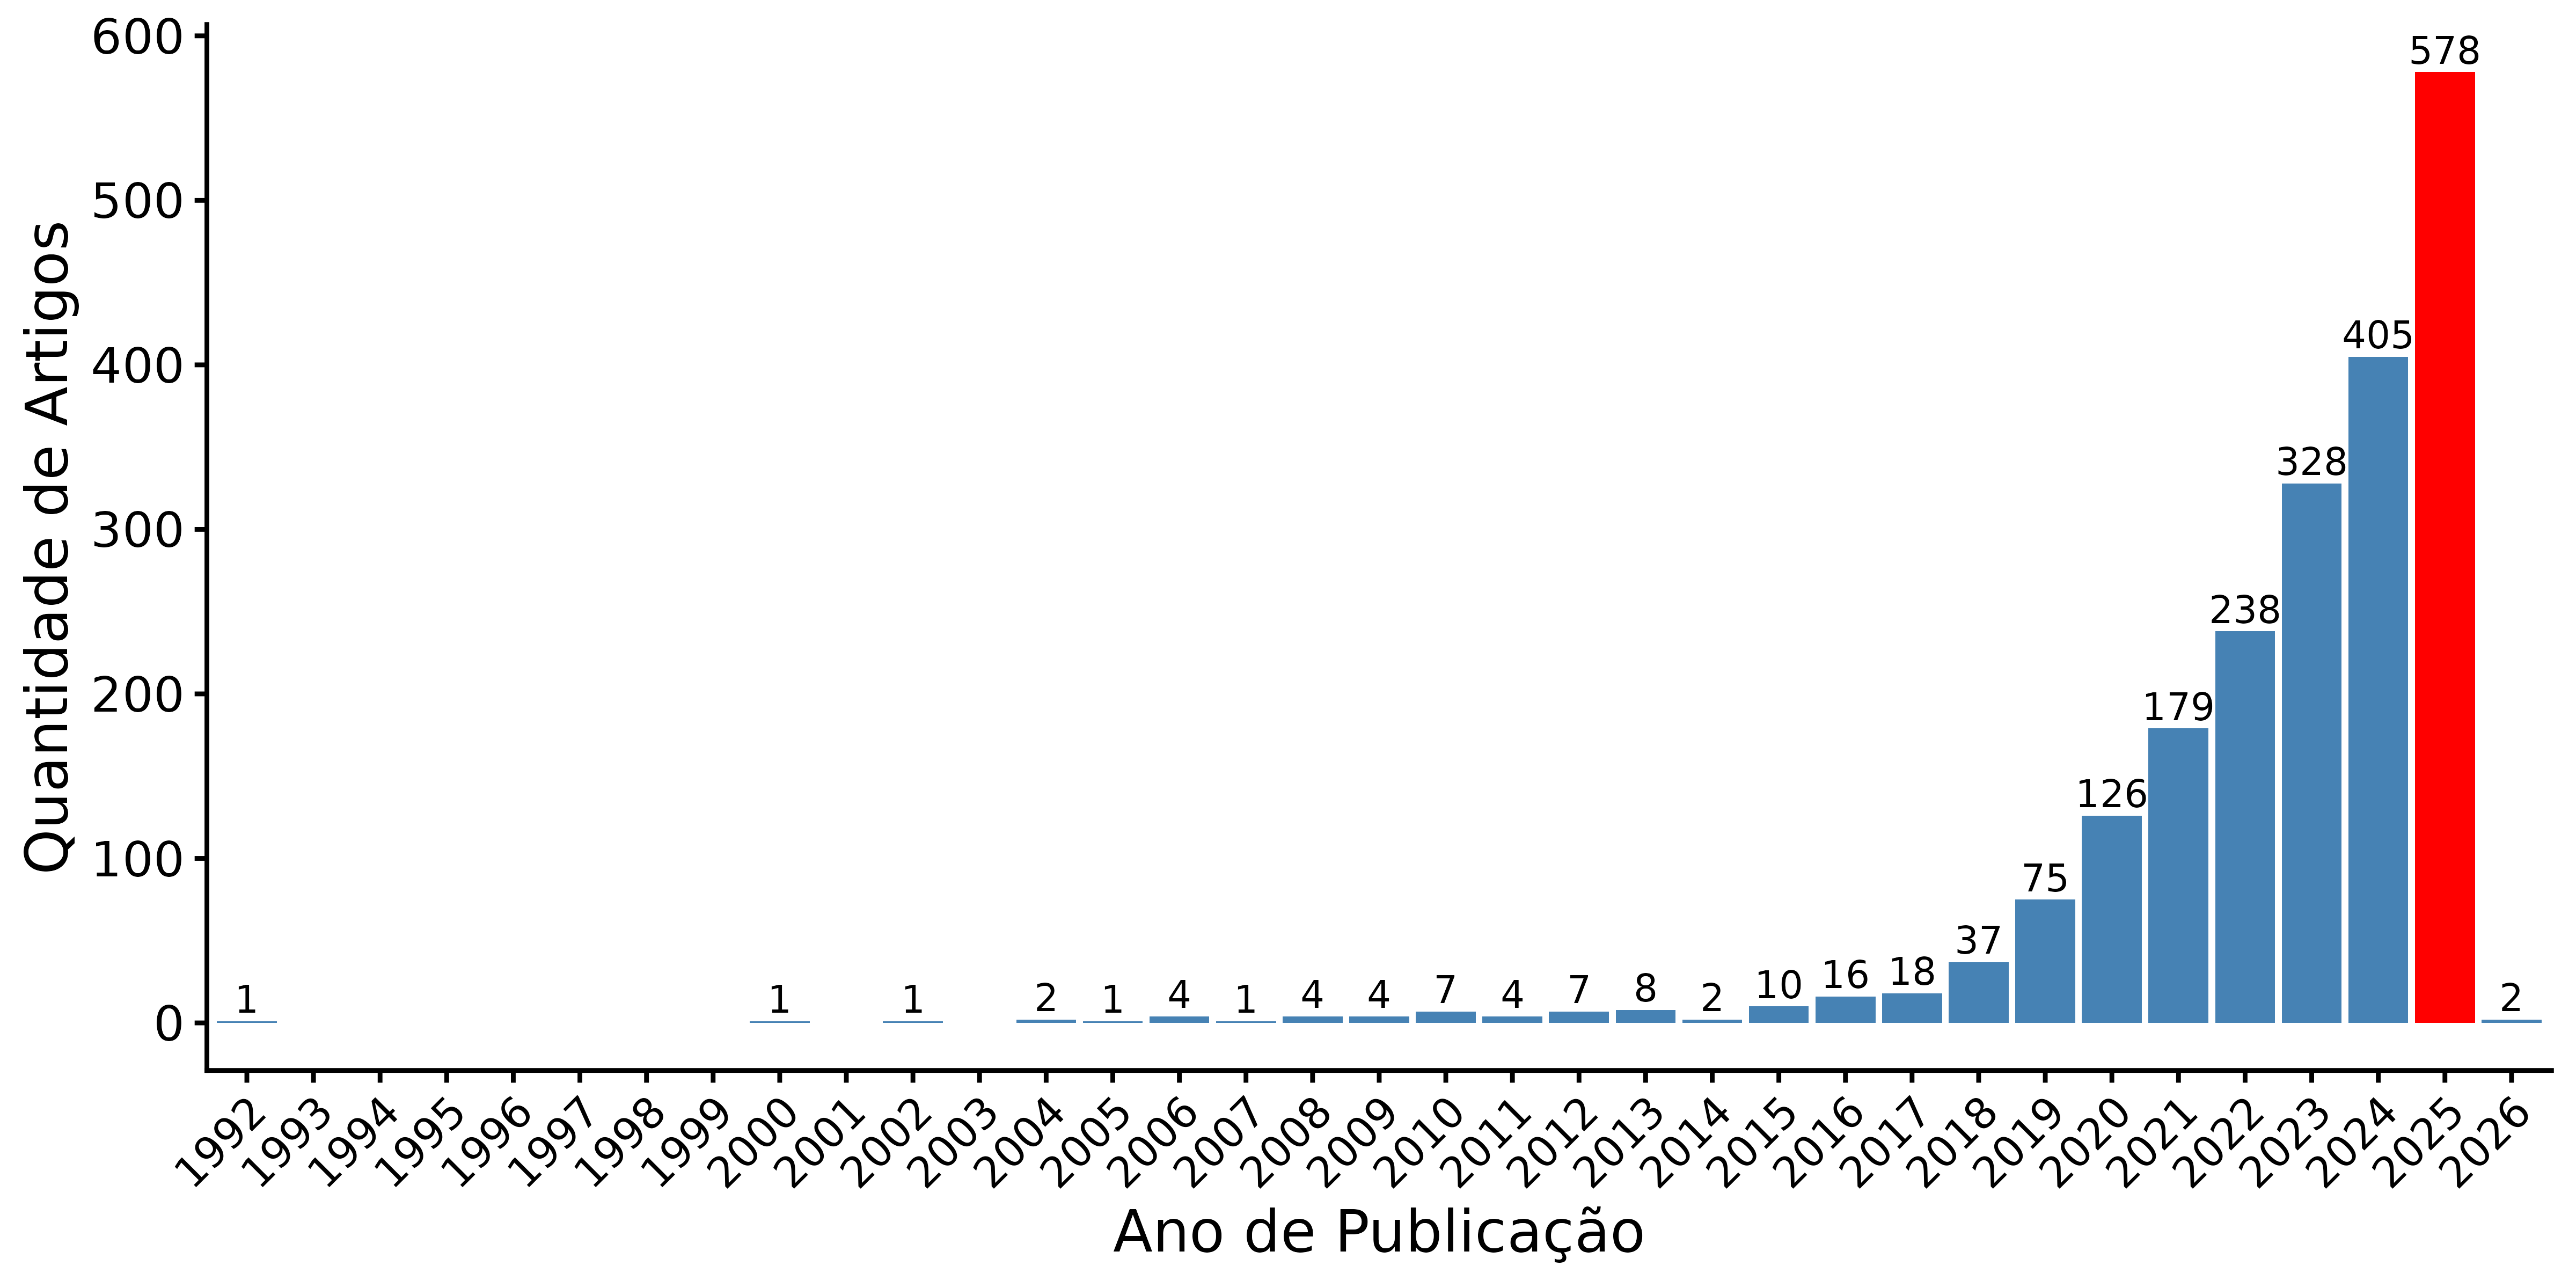
\includegraphics[width=\linewidth]{imagens/sepoc-fig2a-producao.png}
  \caption{Produção anual}
  \label{fig:producao}
\end{subfigure}\hfill
\begin{subfigure}[t]{0.49\textwidth}
  \centering
  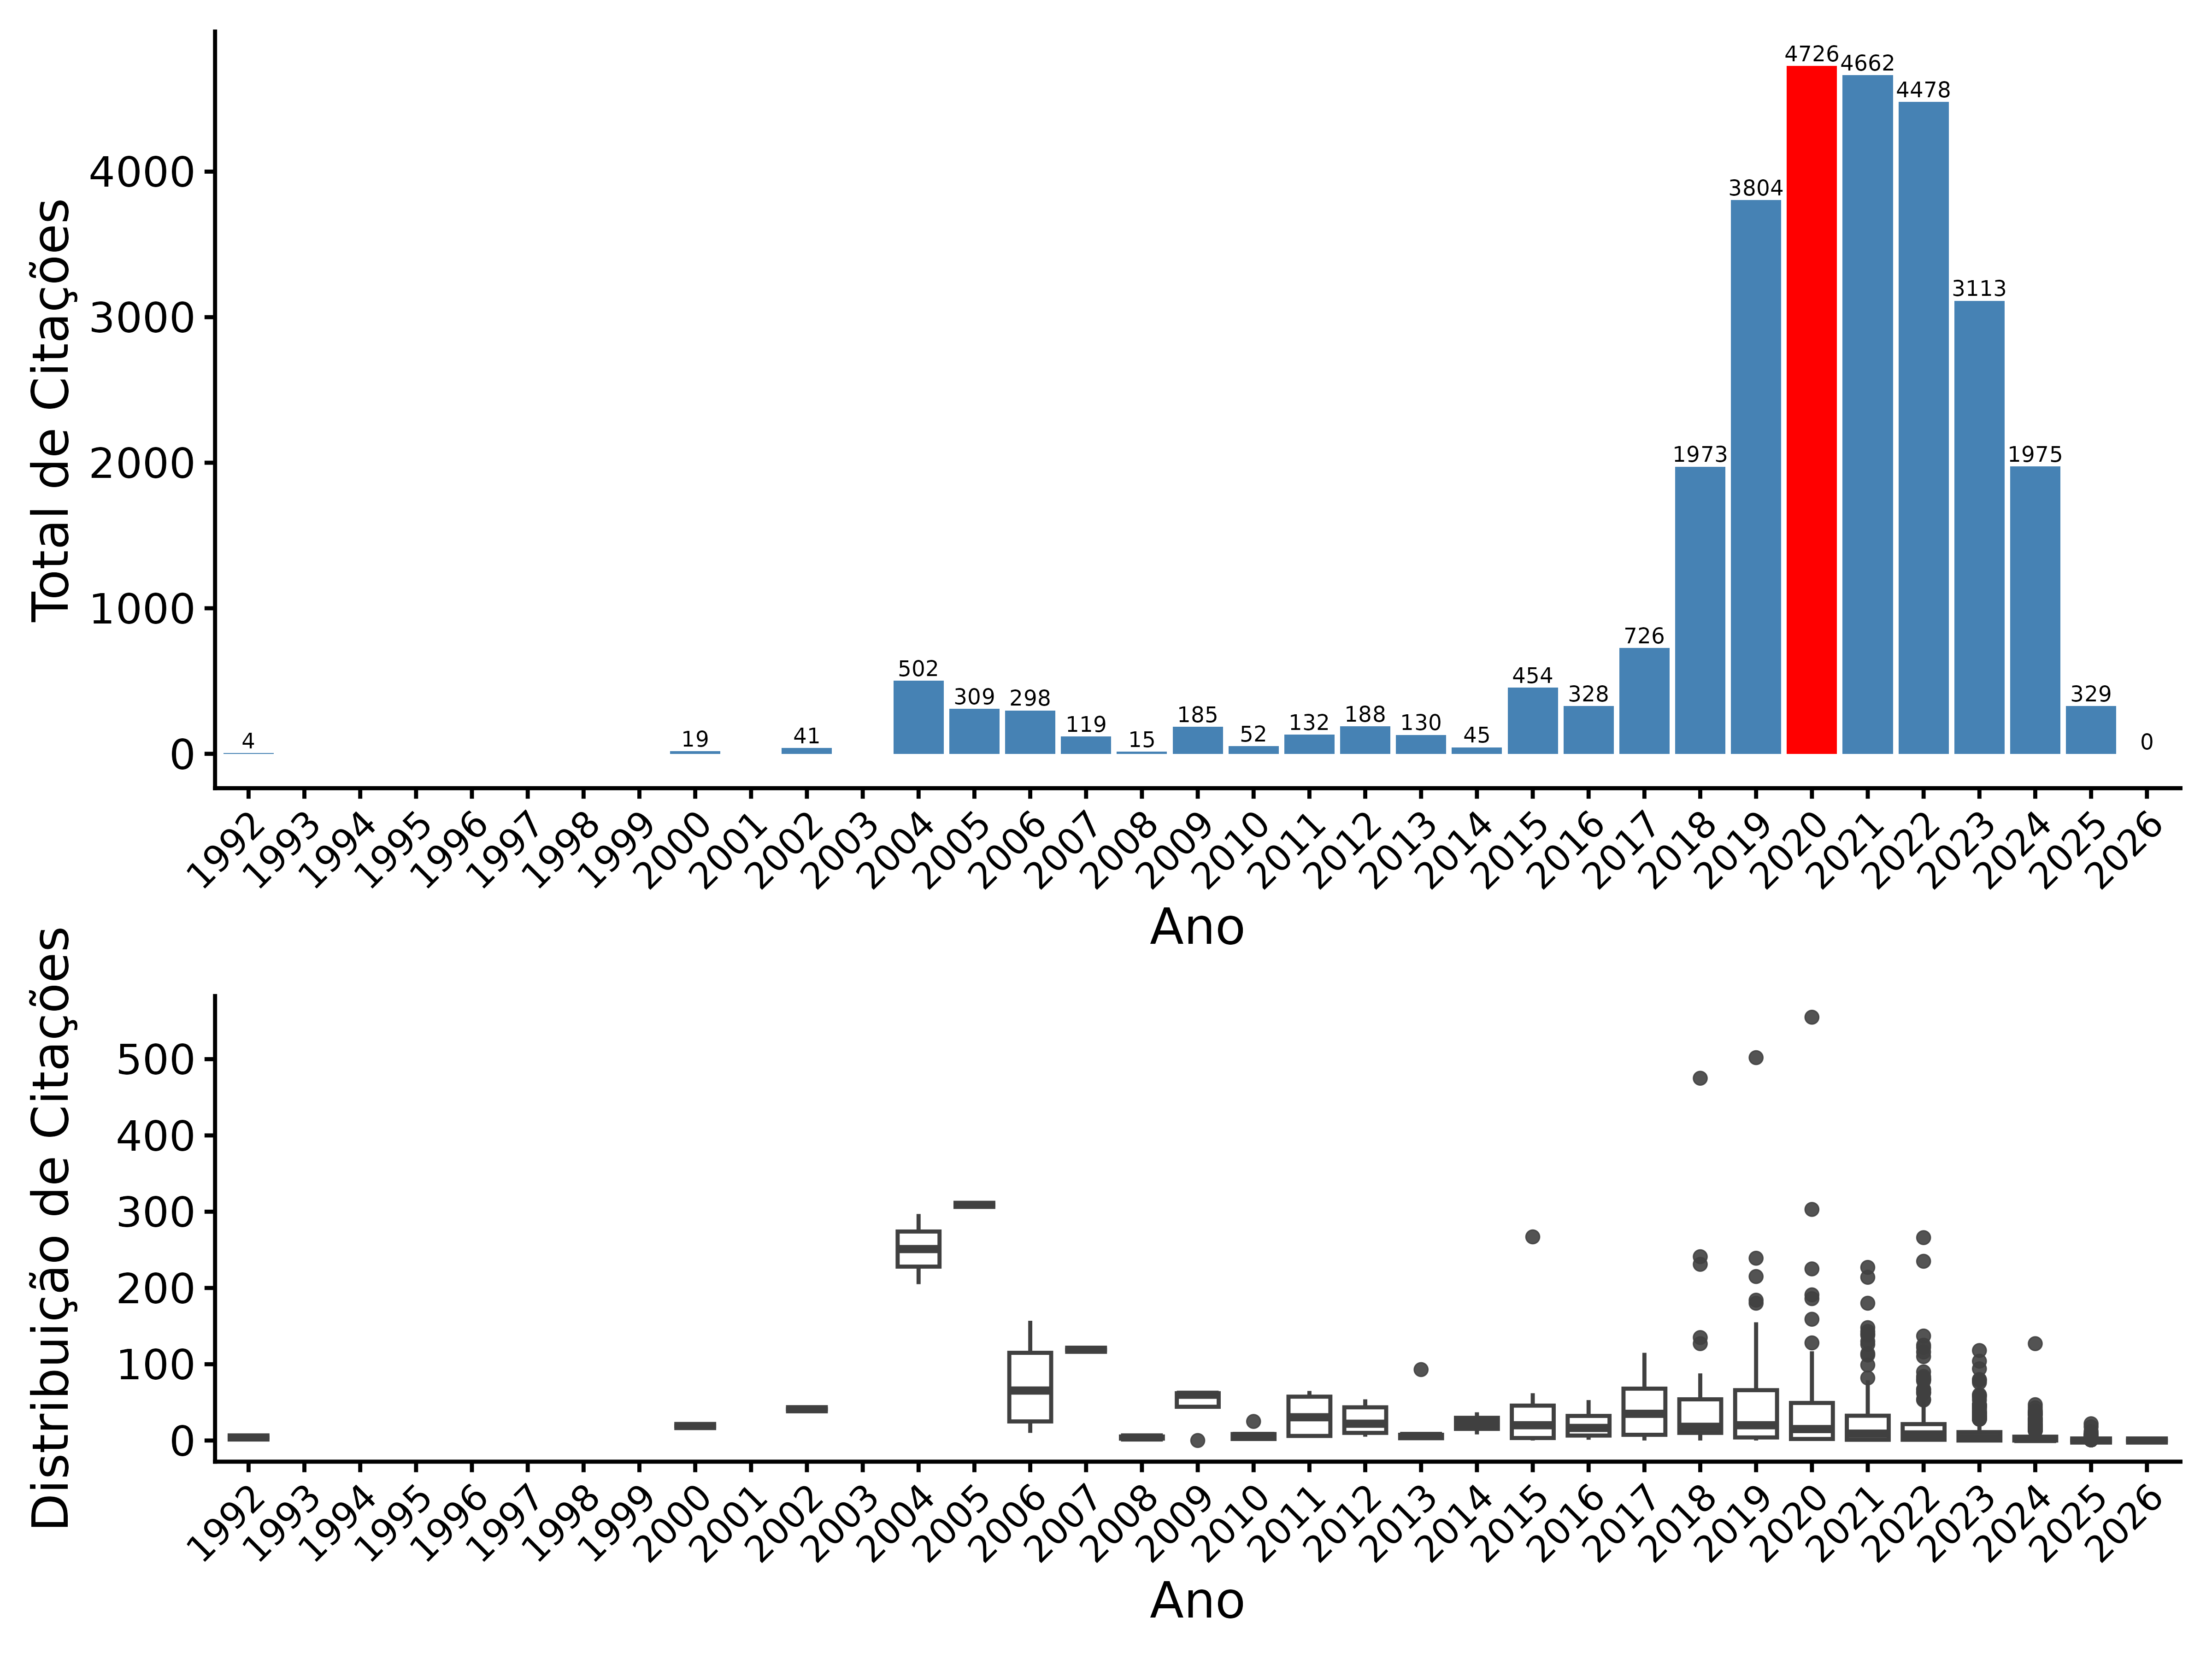
\includegraphics[width=\linewidth]{imagens/sepoc-fig2b-citacoes.png}
  \caption{Citações por ano}
  \label{fig:citacoes}
\end{subfigure}\\[2mm]
{\small Fonte: Elaborado pelos autores.}
\end{figure}

\subsection{Tecnologias e técnicas predominantes}

Entre 2018 e 2025, as categorias de DL e de ML clássico cresceram em ritmo semelhante (cerca de 23 vezes) e os métodos \textit{ensemble}, em ritmo maior (cerca de 33 vezes), partindo de bases pequenas; em números absolutos, o DL é a categoria mais frequente (Figura~\ref{fig:categorias}). Como as categorias são não excludentes, as frequências anuais podem superar o número de documentos do mesmo ano. A queda observada em 2026 é artefato do período parcial.

\textit{Machine learning} foi o termo mais frequente (1.151 ocorrências), seguido por \textit{neural network} (674), \textit{deep learning} (551), Random Forest (358), LSTM (313), \textit{ensemble} (252), CNN (223) e SVM (204) (Figura~\ref{fig:termos}). Transformers e GRU apresentaram frequências menores, compatíveis com tecnologias emergentes no período analisado. A persistência de Random Forest e SVM sugere que métodos clássicos continuam competitivos em bases de dados tabulares e em tarefas de classificação espacial, nas quais interpretabilidade, amostras moderadas e custo computacional permanecem relevantes.

\begin{figure}[!htb]
\centering
\caption{Perfil tecnológico do corpus. As contagens são frequências de ocorrência em metadados harmonizados e não representam conjuntos mutuamente exclusivos de artigos.}
\label{fig:perfil}
\begin{subfigure}[t]{0.52\textwidth}
  \centering
  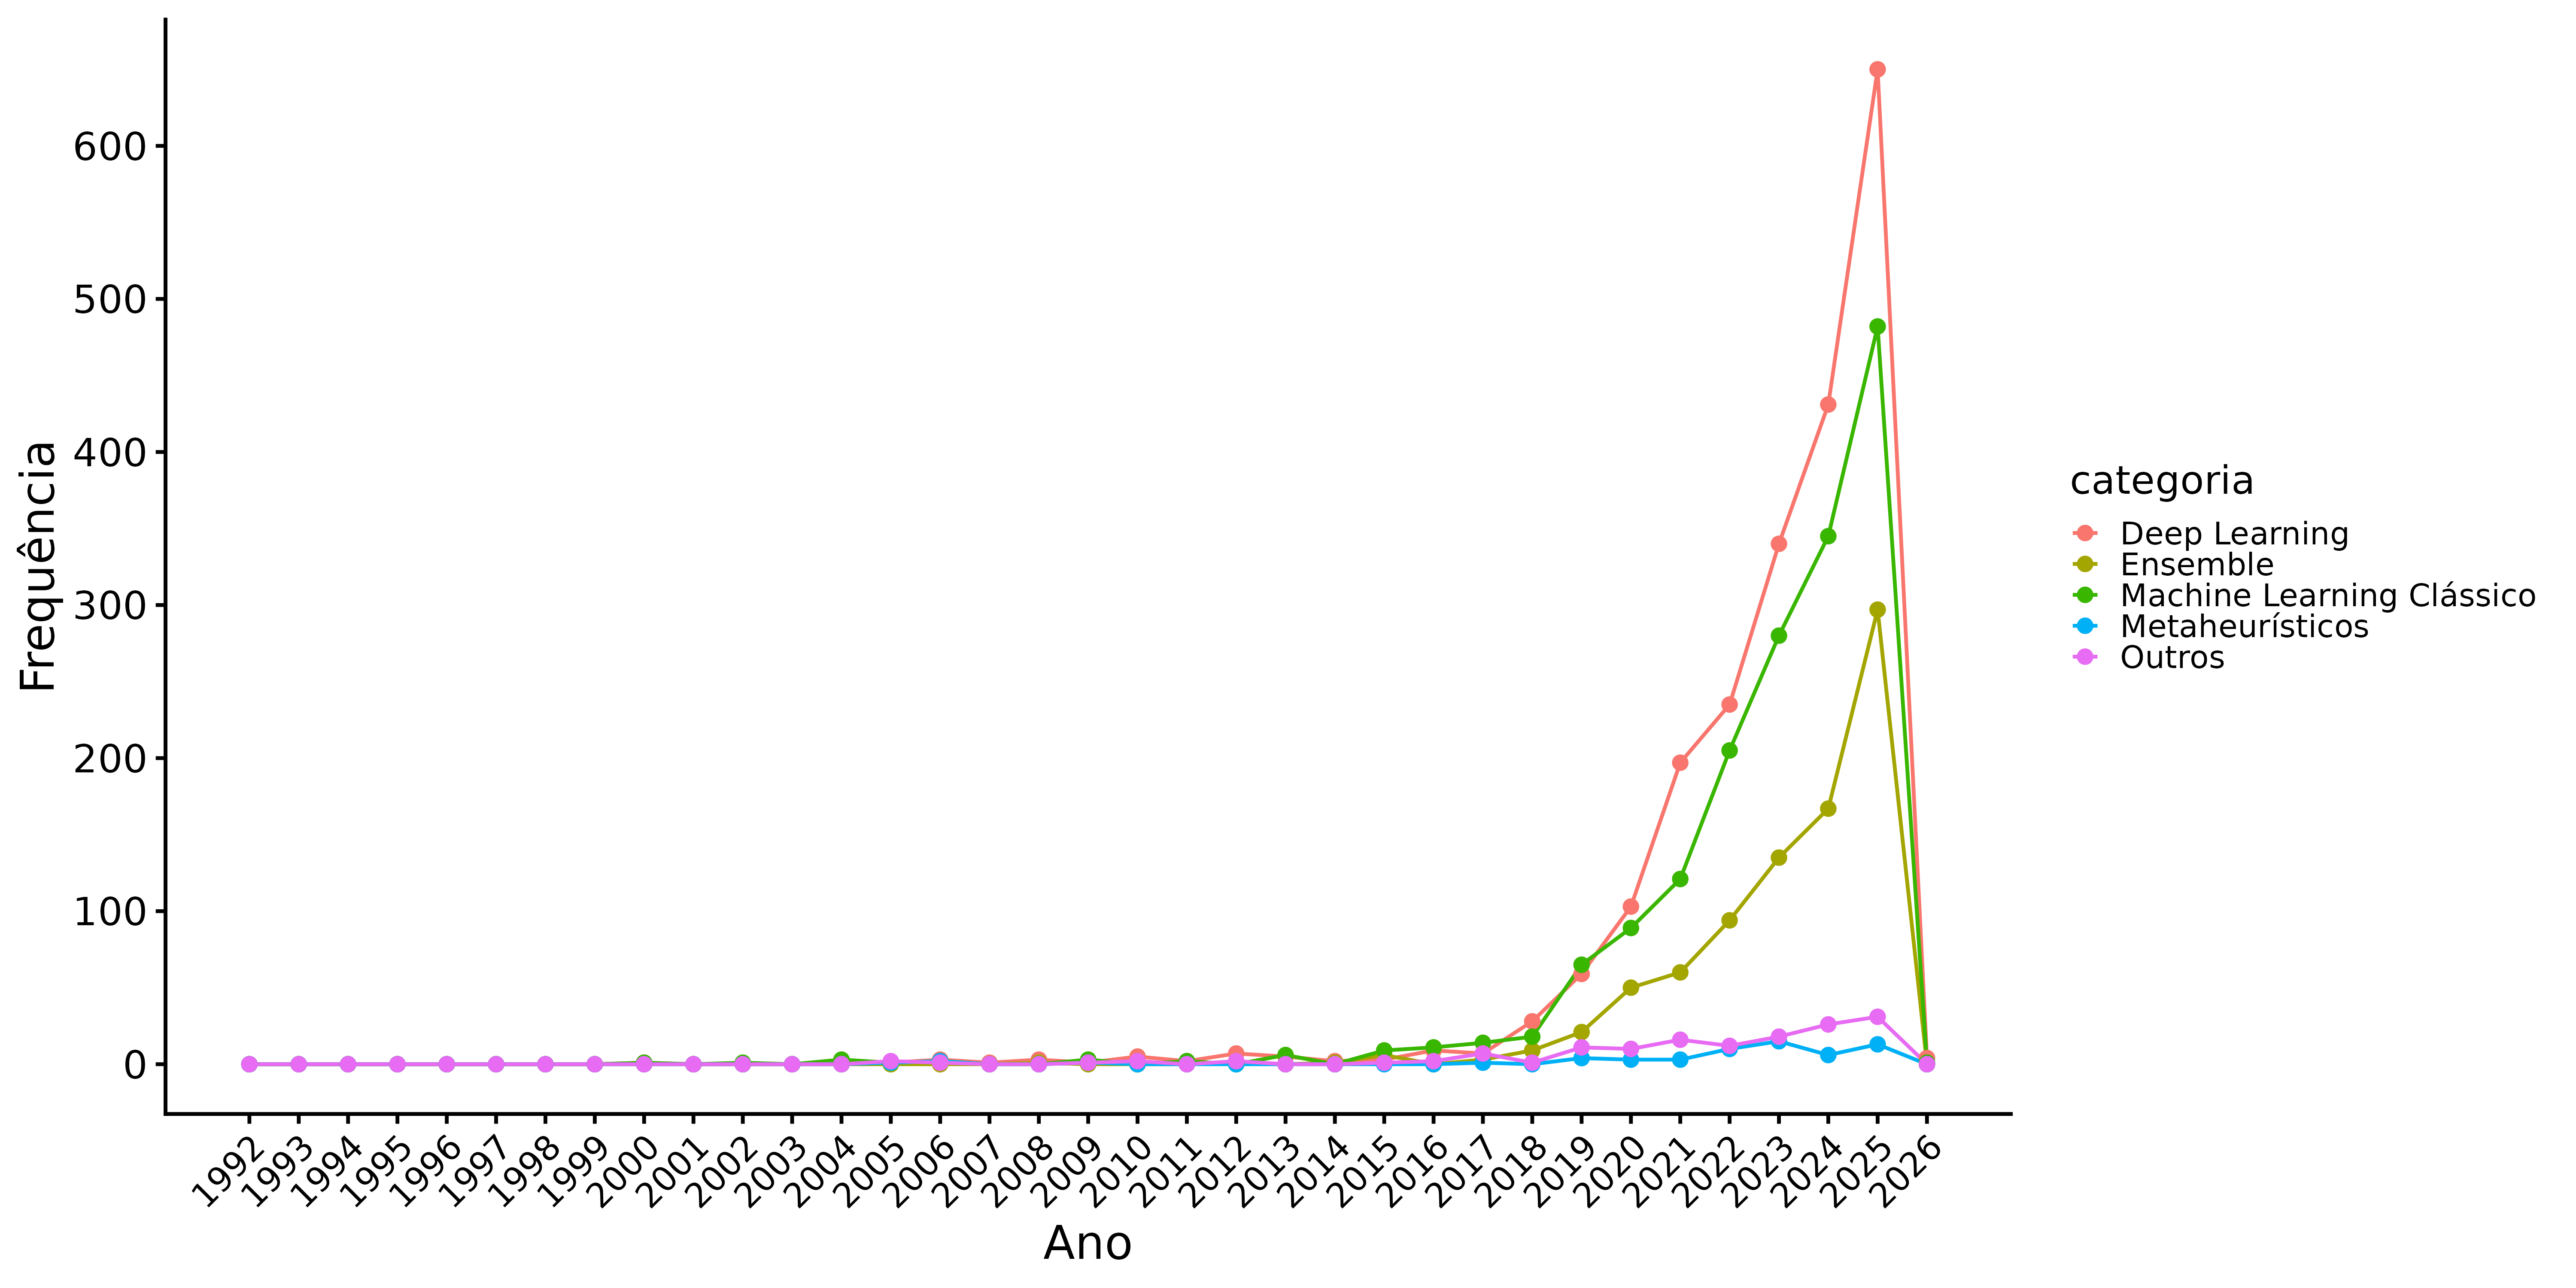
\includegraphics[width=\linewidth]{imagens/sepoc-fig3a-categorias.png}
  \caption{Categorias tecnológicas}
  \label{fig:categorias}
\end{subfigure}\hfill
\begin{subfigure}[t]{0.46\textwidth}
  \centering
  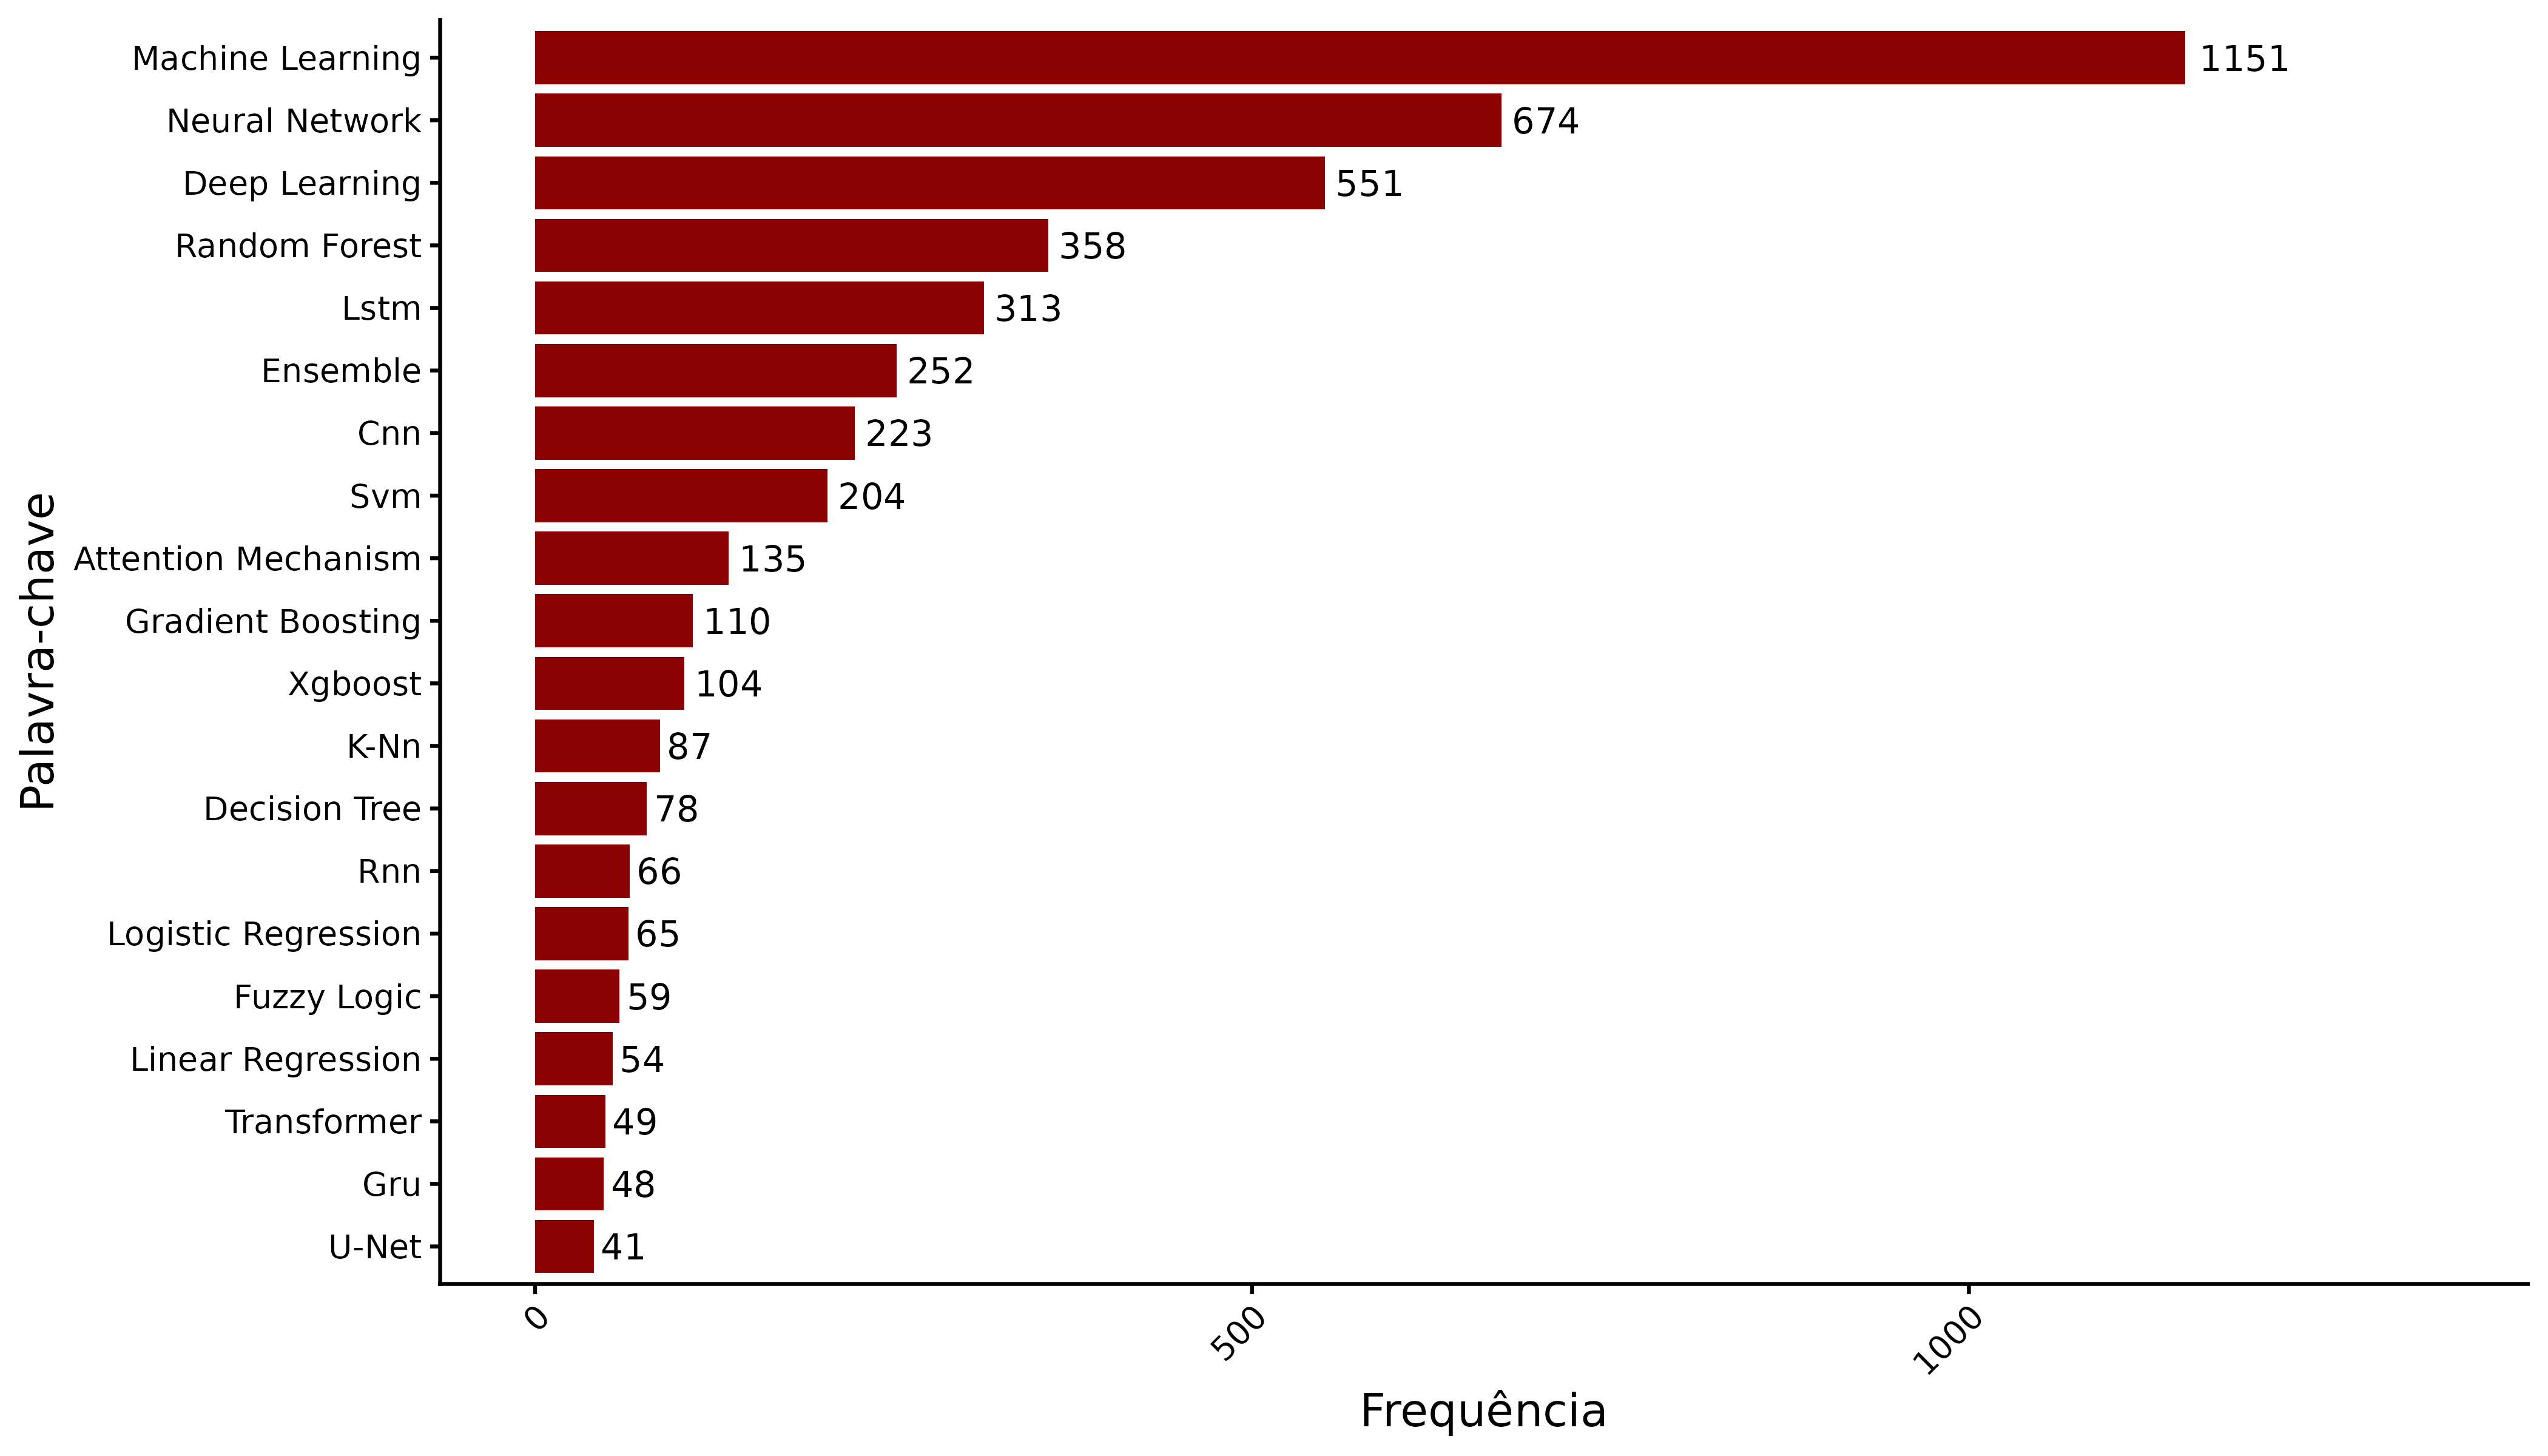
\includegraphics[width=\linewidth]{imagens/sepoc-fig3b-termos.png}
  \caption{Técnicas e termos mais frequentes}
  \label{fig:termos}
\end{subfigure}\\[2mm]
{\small Fonte: Elaborado pelos autores.}
\end{figure}

\subsection{Estrutura temática e evolução das categorias tecnológicas}
\label{sec:art-estrutura}

A rede de coocorrência de palavras-chave calculada pela ferramenta de análise reuniu 614 termos e 7.864 pares e foi dividida em oito agrupamentos pelo método de Louvain (Figura~\ref{fig:mapa}). No mapa temático, quatro agrupamentos ficaram acima das medianas de centralidade e de densidade (quadrante ``motor''): (1) inundações, controle de cheias e \textit{deep learning} (175 termos); (2) \textit{machine learning}, sistemas de aprendizado e previsão de inundações (172); (3) \textit{flooding}, redes neurais artificiais e China (98); e (4) avaliação de risco e mudança climática (77). O agrupamento de sensoriamento remoto, redes neurais convolucionais e inundação urbana (70 termos) ficou abaixo das medianas (quadrante ``emergente ou em declínio''), assim como os de lógica difusa e otimização (10), de umidade do solo (10) e um agrupamento residual (2). Como o mapa usa os termos tal como constam nas bases, variantes de grafia (``machine learning'' e ``machine-learning'') permanecem separadas; ao unificá-las, os agrupamentos passam de oito para seis e, ao normalizar também hífen e espaço, para sete. A partição é, portanto, sensível à normalização das palavras-chave e é apresentada como descrição exploratória, sem inferência sobre fronteiras temáticas estáveis.

\begin{figure}[!htb]
\centering
\caption{Mapa temático dos agrupamentos de palavras-chave. Cada círculo é um agrupamento, numerado conforme o texto, com área proporcional à frequência de seus termos. As linhas tracejadas indicam as medianas de centralidade e de densidade; em azul, o quadrante ``motor''; em vermelho, o quadrante ``emergente ou em declínio''.}
\label{fig:mapa}
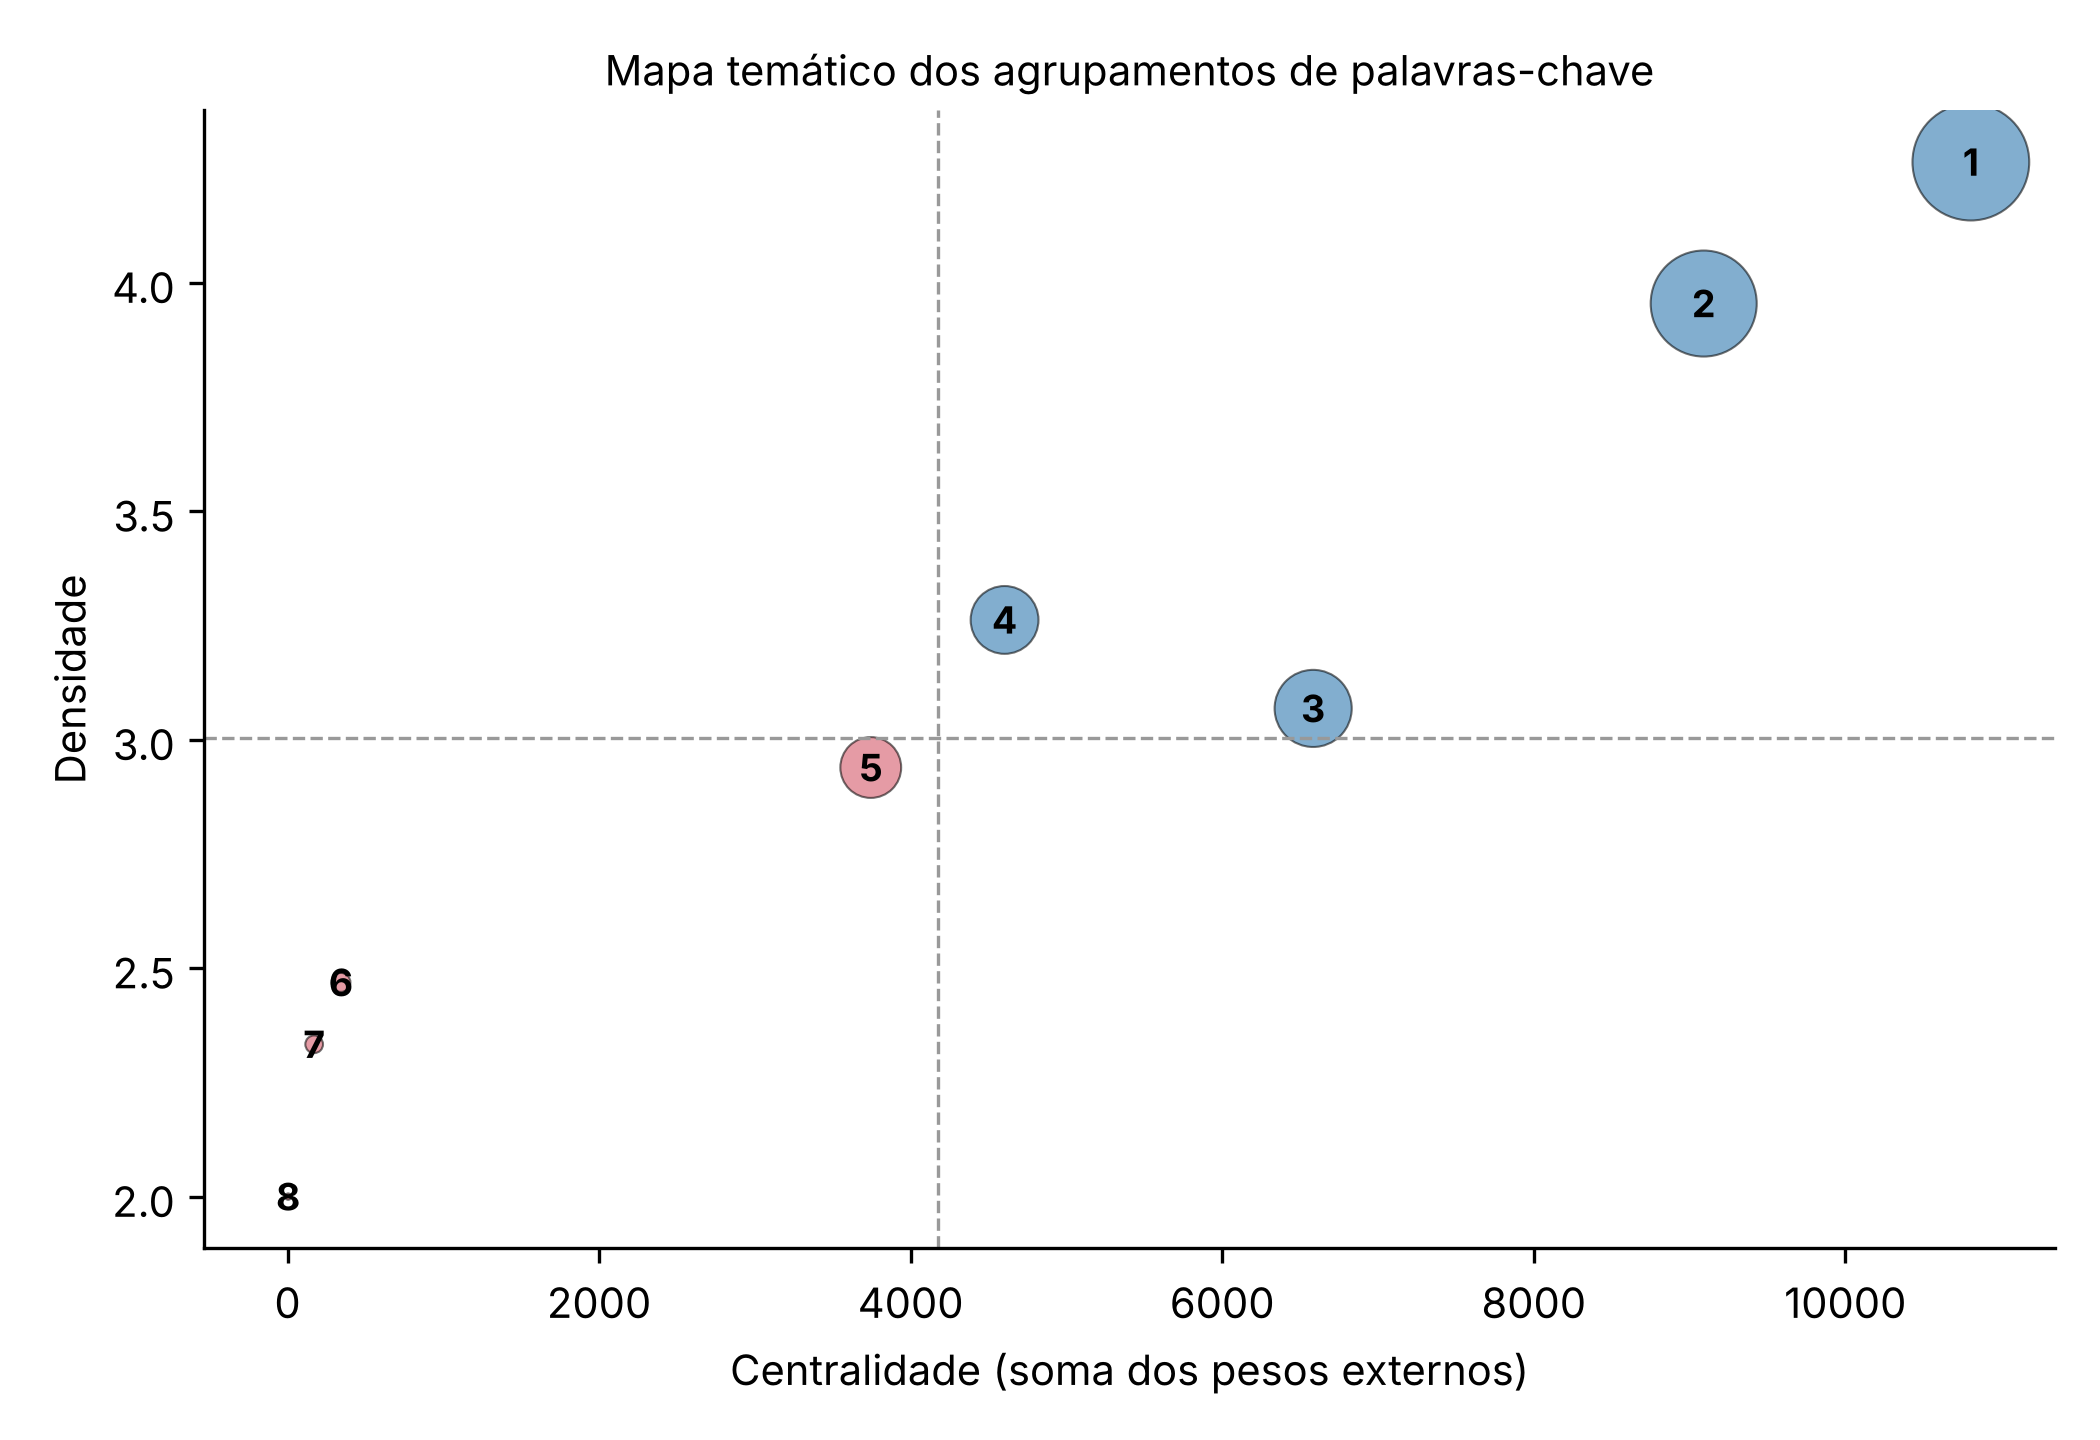
\includegraphics[width=0.75\textwidth]{imagens/sepoc-fig6-mapa-tematico.png}\\[2mm]
{\small Fonte: Elaborado pelos autores.}
\end{figure}

A Figura~\ref{fig:tecano} mostra a frequência anual de três categorias de métodos. Entre 2018 e 2025, as ocorrências de \textit{deep learning} passaram de 27 para 622, as de \textit{machine learning} clássico de 23 para 523 e as de \textit{ensemble} de 9 para 293. Em participação no total de ocorrências, porém, o \textit{deep learning} oscilou entre 30,0\% e 46,3\% sem tendência monotônica (42,6\% em 2025), o \textit{machine learning} clássico passou de 38,3\% para 35,8\% e o \textit{ensemble}, de 15,0\% para 20,1\%. O crescimento observado reflete, assim, principalmente o aumento do volume de publicações, e não a substituição de uma categoria por outra. O \textit{deep learning} superou o \textit{machine learning} clássico em frequência em 2021 e a partir de 2023, mas não em 2022 (217 contra 224). As categorias não são excludentes, 2026 foi omitido por ser ano parcial, e a harmonização de termos da ferramenta difere da usada na Figura~\ref{fig:perfil} (por exemplo, \textit{machine learning} soma 1.273 ocorrências na ferramenta e 1.151 na outra contagem).

\begin{figure}[!htb]
\centering
\caption{Evolução das categorias tecnológicas, 2018--2025. As categorias não são excludentes. Em (b), a participação é calculada sobre o total de ocorrências das cinco categorias da ferramenta (inclui metaheurísticos e outros).}
\label{fig:tecano}
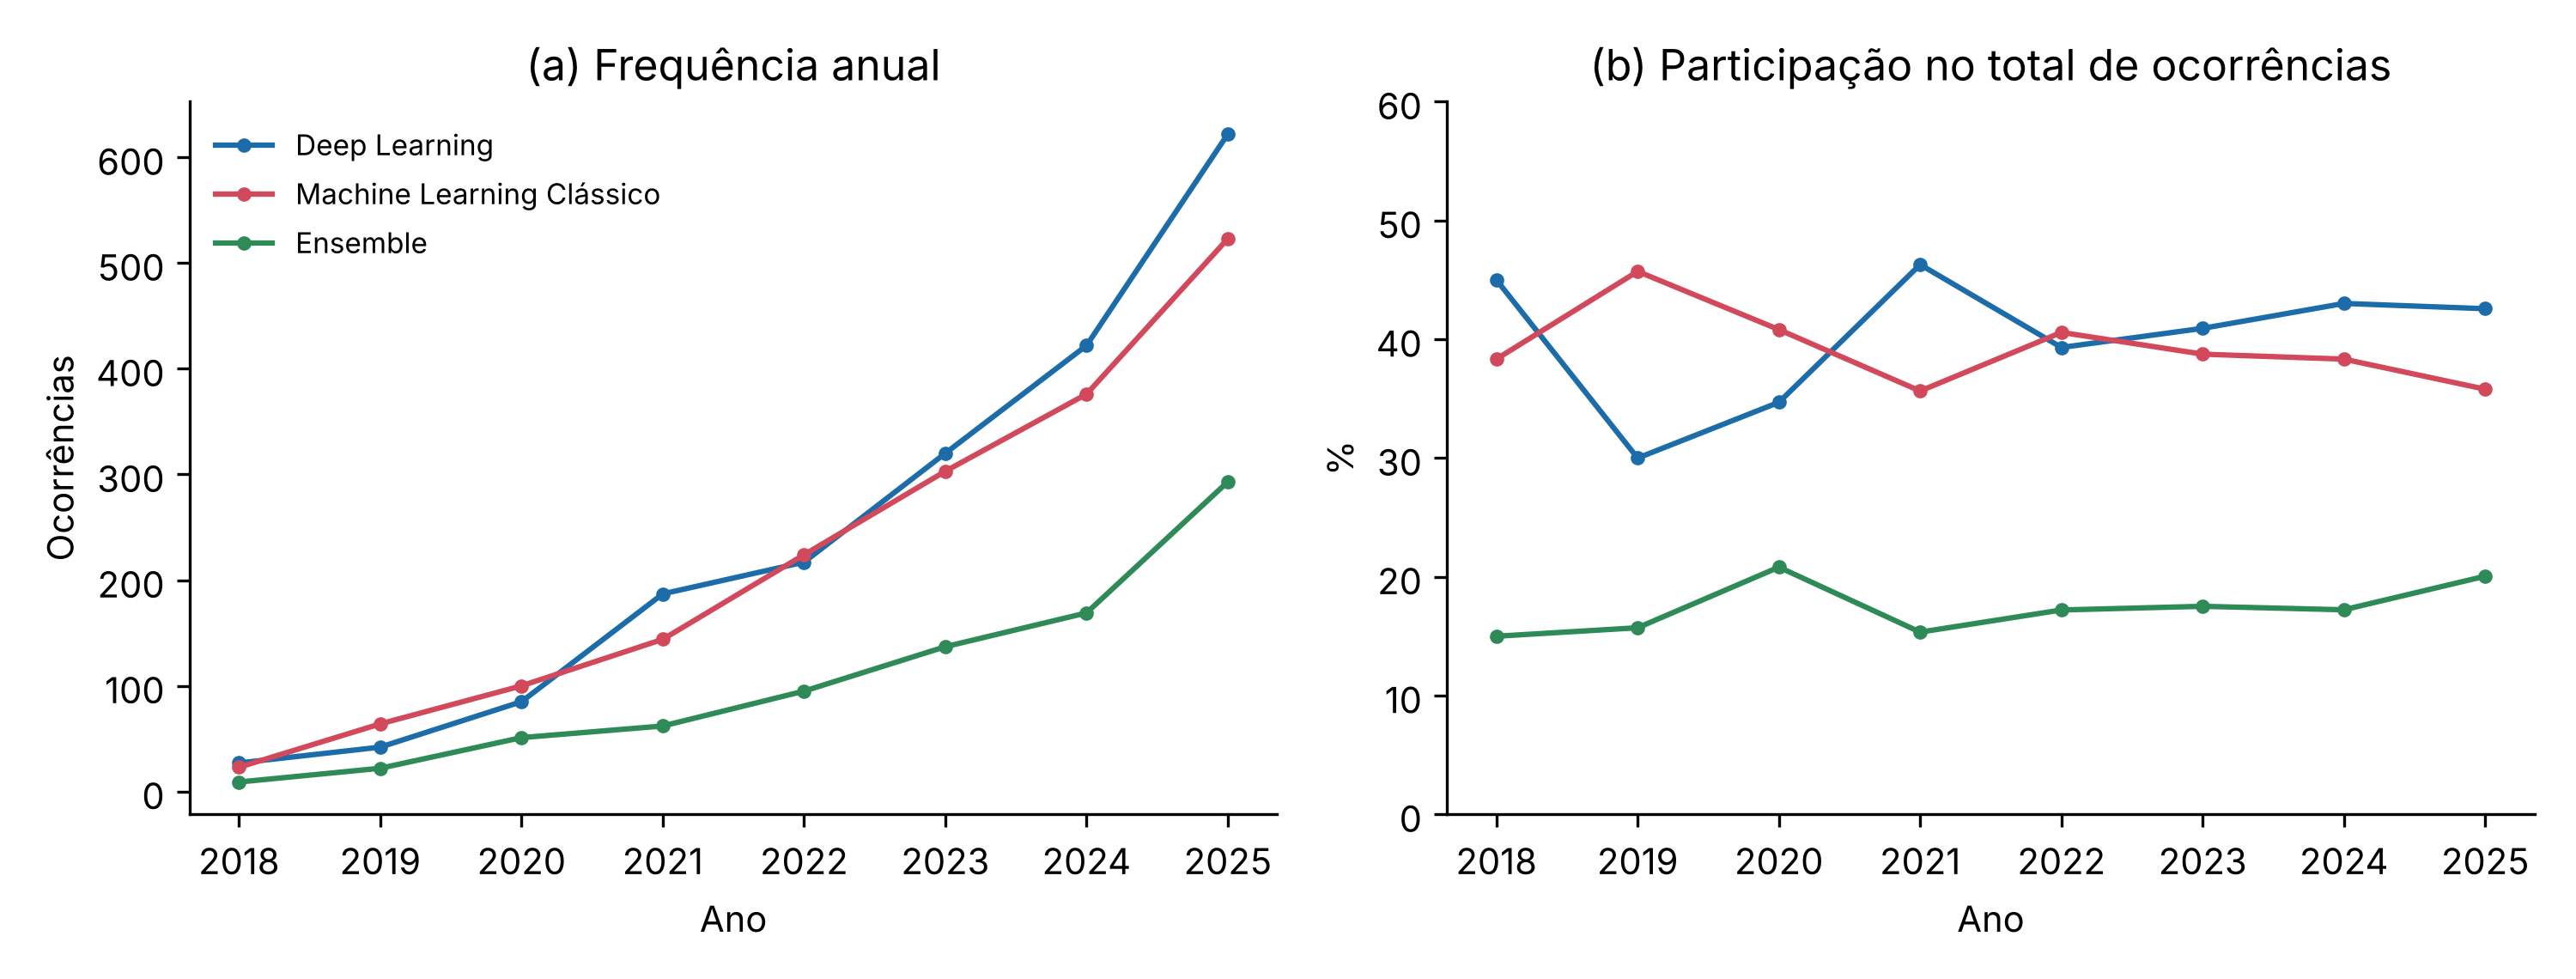
\includegraphics[width=\textwidth]{imagens/sepoc-fig5-tecnologias-ano.png}\\[2mm]
{\small Fonte: Elaborado pelos autores.}
\end{figure}

\subsection{Distribuição geográfica}

A China apresentou o maior número de publicações por afiliação (364), seguida por Estados Unidos (119) e Índia (117). Irã, Taiwan, Canadá e Vietnã também se destacaram (Figura~\ref{fig:paises}). Brasil e outros países latino-americanos não figuraram entre os 20 primeiros. Esse resultado sugere sub-representação no corpus recuperado, mas não comprova ausência de estudos, pois depende da estratégia de busca, da cobertura das bases, do idioma e do método de contagem de afiliações.

\begin{figure}[!htb]
\centering
\caption{Países com maior número de publicações segundo os metadados de afiliação. A unidade geográfica não deve ser confundida com o local de aplicação empírica do estudo.}
\label{fig:paises}
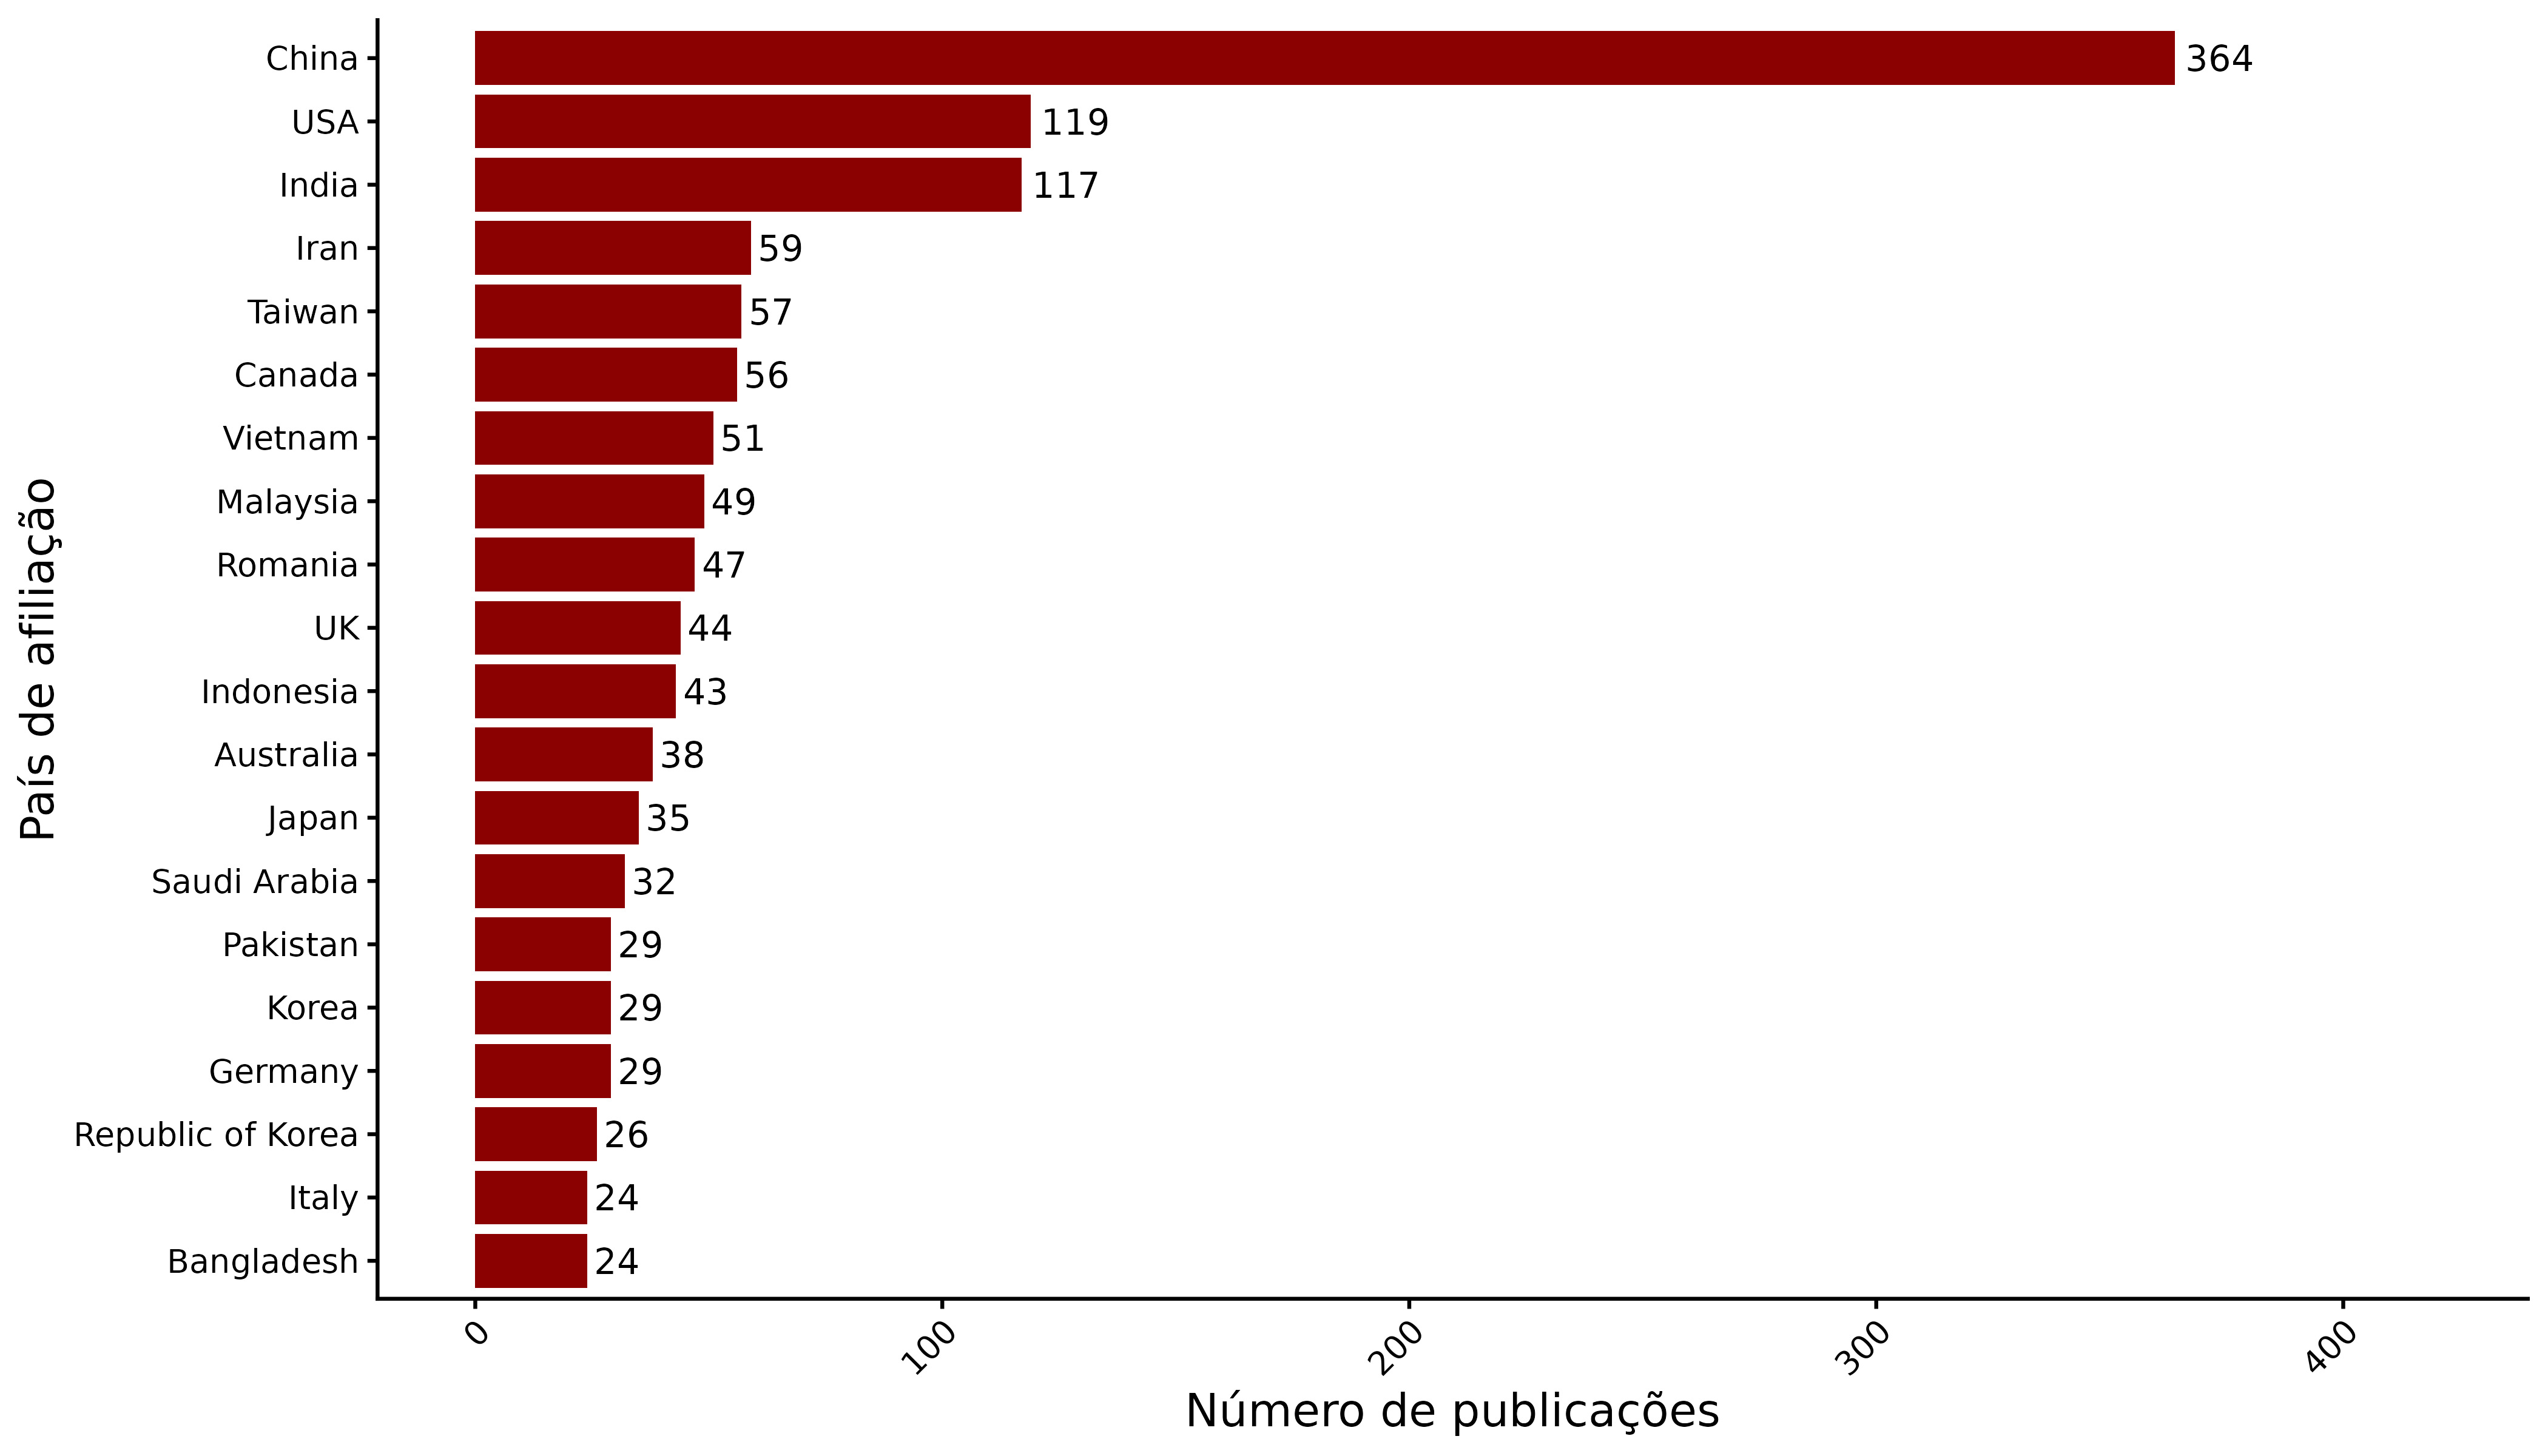
\includegraphics[width=0.75\textwidth]{imagens/sepoc-fig4-paises.png}\\[2mm]
{\small Fonte: Elaborado pelos autores.}
\end{figure}

\subsection{Síntese dos artigos de maior prioridade}

Os 13 artigos do Núcleo A foram publicados entre 2018 e 2021 e apresentaram média de 283 citações na base consolidada. A Tabela~\ref{tab:nucleoA} evidencia que o estrato não é composto apenas por previsão temporal, predominam o mapeamento de suscetibilidade, a classificação espacial e a integração com sensoriamento remoto. Essa composição explica a coexistência de métricas hidrológicas, como NSE e R$^2$, com métricas de classificação, como AUC, acurácia, sensibilidade e especificidade.

{\small
\renewcommand{\arraystretch}{1.2}
\begin{longtable}{@{}p{2.7cm}p{2.6cm}p{3.1cm}p{5.6cm}@{}}
\caption{Síntese funcional dos 13 artigos do Núcleo A. Valores de desempenho não são comparados porque tarefas, dados, escalas e desenhos de validação diferem entre estudos.}\label{tab:nucleoA}\\
\toprule
\textbf{Estudo} & \textbf{Tarefa principal} & \textbf{Método} & \textbf{Contribuição científica central}\\
\midrule
\endfirsthead
\toprule
\textbf{Estudo} & \textbf{Tarefa principal} & \textbf{Método} & \textbf{Contribuição científica central}\\
\midrule
\endhead
\midrule
\multicolumn{4}{r}{\footnotesize\textit{continua na próxima página}}\\
\endfoot
\bottomrule
\multicolumn{4}{@{}l}{\footnotesize Fonte: Elaborado pelos autores.}\\
\endlastfoot
\citeonline{xiang2020} & Previsão chuva--vazão & LSTM \textit{sequence-to-sequence} & Previsão em múltiplos passos e representação de dependências temporais.\\
\citeonline{tyralis2019} & Revisão metodológica & Random Forest e variantes & Sistematização do uso de florestas aleatórias em recursos hídricos e importância de variáveis.\\
\citeonline{hu2018} & Simulação chuva--vazão & LSTM & Aplicação de memória recorrente à dinâmica hidrológica e aos picos de vazão.\\
\citeonline{janizadeh2019} & Suscetibilidade a enxurradas & ADT, FT, KLR, MLP e QDA & Comparação de classificadores sobre fatores geoambientais.\\
\citeonline{dodangeh2020} & Suscetibilidade & GAM, MARS, BRT e reamostragem & Tratamento do desbalanceamento entre ocorrências e não ocorrências.\\
\citeonline{rafieisardooi2021} & Risco urbano & ML e TOPSIS & Integração entre perigo físico e vulnerabilidade socioeconômica.\\
\citeonline{zhao2019} & Suscetibilidade urbana & WELLSVM semissupervisionado & Aproveitamento de dados não rotulados em inventários incompletos.\\
\citeonline{fang2021} & Suscetibilidade & LSTM & Uso de arquitetura recorrente em padrões espaciais de condicionantes.\\
\citeonline{costache2020} & Suscetibilidade a enxurradas & KNN, AHP e análise multicritério & Integração entre ML, sensoriamento remoto, SIG e decisão multicritério.\\
\citeonline{shahabi2020} & Detecção e suscetibilidade & Sentinel-1 e \textit{ensemble} Bagging--KNN & Combinação de velocidade da Terra com classificadores \textit{ensemble}.\\
\citeonline{arora2021} & Suscetibilidade & ANFIS com GA, DE e PSO & Otimização metaheurística de modelos neurodifusos.\\
\citeonline{wu2020} & Revisão de previsão & Previsão probabilística \textit{ensemble} & Ênfase em incerteza, assimilação de dados e uso operacional.\\
\citeonline{saha2021} & Suscetibilidade & Hyperpipes, SVR e \textit{ensemble} HP--SVR & Combinação de algoritmos com perfis complementares de classificação.\\
\end{longtable}
}

% ---------------------------------------------------------------------
\section{Discussão}
\label{sec:art-discussao}

\subsection{Crescimento bibliométrico não equivale à maturidade operacional}

O aumento de publicações revela forte mobilização científica, mas não demonstra, isoladamente, ganho em termos de generalização, robustez ou utilidade operacional. Parte do crescimento decorre da expansão dos dados de sensoriamento remoto, das reanálises meteorológicas, dos sensores de baixo custo e da infraestrutura computacional. O avanço mais relevante ocorre quando modelos são avaliados fora da amostra, em bacias, períodos e extremos não utilizados no treinamento. O sistema global analisado por \citeonline{nearing2024} empregou validação espacial e temporal explícita e comparação com um sistema operacional de referência, oferecendo um padrão mais exigente do que o de divisões aleatórias de treino e teste.

\subsection{A tarefa científica deve preceder a escolha do algoritmo}

A principal fragilidade conceitual do corpus é o uso indiscriminado de ``previsão de inundação'' para tarefas distintas. A previsão hidrológica estima estados futuros e requer horizonte de antecedência, persistência, erro de pico, NSE, KGE, viés e calibração probabilística. Mapeamento de suscetibilidade estima a propensão espacial e costuma empregar AUC, sensibilidade, especificidade e acurácia. A detecção de inundação segmenta áreas afetadas em imagens e requer métricas como IoU e F1. Avaliação de risco combina perigo, exposição e vulnerabilidade, não podendo ser reduzida à acurácia de um classificador.

Consequentemente, valores elevados de AUC em um mapa de suscetibilidade não podem ser interpretados como evidência de capacidade de alerta em tempo real; da mesma forma, um bom NSE médio não garante reprodução dos extremos que interessam à defesa civil. Comparações futuras devem ser estratificadas por tarefa, escala, horizonte, fonte de dados e protocolo de validação.

\subsection{Validação, dependência espacial e incerteza}

Dados hidrológicos e geoespaciais apresentam autocorrelação temporal e espacial. Divisões aleatórias podem colocar observações muito semelhantes nos conjuntos de treino e teste, produzindo estimativas otimistas de desempenho. A validação bloqueada no espaço, no tempo e por evento, bem como testes em bacias não observadas, são necessários para avaliar a transferência real \cite{roberts2017}. Para aplicações operacionais, recomenda-se comparar a IA com referências simples e modelos físicos, reportar o desempenho por horizonte e por magnitude do evento, quantificar a incerteza e avaliar a calibração probabilística.

Modelos híbridos e guiados por conhecimento oferecem uma direção promissora, pois podem combinar flexibilidade estatística com restrições de balanço hídrico, de conectividade de drenagem e de coerência física \cite{nearing2021}. A interpretabilidade também deve ser tratada como requisito de segurança e de diagnóstico, e não apenas como recurso de visualização posterior.

\subsection{Lacuna costeira, desigualdade de dados e aplicabilidade regional}

A baixa representação latino-americana e a ausência de contextos costeiros brasileiros no Núcleo A são relevantes, mas precisam ser interpretadas com cautela. A própria expressão de busca privilegia termos genéricos e urbanos e não inclui explicitamente vocabulário de inundação costeira ou composta. Assim, parte da lacuna observada é substantiva e outra pode ser decorrente do desenho da busca.

Em municípios costeiros, modelos devem integrar precipitação, nível do rio, maré, sobreelevação meteorológica, ondas, impermeabilização e capacidade da drenagem. A análise isolada desses componentes pode subestimar eventos compostos \cite{wahl2015}. Para cidades médias e regiões com monitoramento limitado, a agenda mais promissora combina sensores locais, radar meteorológico, produtos de satélite, reanálises, modelos hidrodinâmicos simplificados e IA com transferência entre bacias. Dados abertos e protocolos comuns de validação são fundamentais para reduzir a desigualdade entre regiões bem monitoradas e áreas altamente vulneráveis.

\subsection{Agenda de pesquisa}

Os resultados sustentam cinco prioridades: (i) ampliar a estratégia de busca com vocabulário costeiro, composto e operacional; (ii) separar análises por tarefa científica; (iii) adotar validação espaço-temporal e por eventos extremos; (iv) combinar previsão pontual com incerteza, interpretabilidade e coerência física, e; (v) disponibilizar exportações, dicionários de palavras-chave, código de deduplicação e cálculo do escore, e reprocessar o corpus com a exclusão restrita a palavras inteiras, o mapeamento de colunas corrigido e a proveniência por base preservada, o que recuperaria registros como \citeonline{mosavi2018}. A tendência de adoção de Transformers e arquiteturas mais profundas é relevante. Entretanto, a maior complexidade dos modelos deve ser acompanhada por protocolos rigorosos de validação. Quando informações do período, local ou evento usado para avaliação também influenciam o treinamento, a potencial ocorrência de \textit{data leakage} passa a ser aumentada, produzindo assim estimativas artificialmente elevadas de desempenho e pouca capacidade de generalização do modelo e detecção de novas enchentes.

% ---------------------------------------------------------------------
\section{Limitações}
\label{sec:art-limitacoes}

Algumas limitações condicionam a interpretação dos resultados. Primeiro, a triagem foi automatizada, sem avaliação manual por revisores, e depende de correspondência lexical de termos, que perde sinônimos e pode aceitar termos polissêmicos; a única verificação manual realizada foi a conferência, pela autora, dos 13 artigos do Núcleo A. Segundo, a cobertura da busca é parcial: na validação externa, apenas metade das referências internacionais de \citeonline{dias2025} estava entre os registros recuperados, e a expressão de busca não abrangeu a totalidade de sinônimos de inundações pluviais, repentinas, costeiras e compostas. Terceiro, o escore é relativo ao corpus (reescala por mínimo e máximo): o valor 100 identifica o artigo de maior escore neste corpus, e não qualidade absoluta. Além disso, o escore, cujos pesos e cortes foram adotados sem calibração própria, favorece artigos mais antigos pelo peso das citações, e o corte fixo do Núcleo A é sensível aos pesos e à composição do corpus, embora o ranking seja mais estável a variações moderadas. Quarto, o procedimento tem falhas de implementação documentadas: o mapeamento de colunas não reconheceu títulos do IEEE Xplore e campos da SciELO, de modo que o corpus provém, na prática, da Lens e da Scopus; 539 registros sem DOI foram descartados como se fossem duplicatas; a proveniência por base não foi preservada; e a exclusão por trecho de texto removeu 498 registros pertinentes (Seção~\ref{sec:art-sensibilidade}); o casamento por trecho também afeta termos de contexto (por exemplo, \textit{rio} dentro de \textit{various}), e 27 pares de DOIs que diferem apenas na caixa permanecem duplicados no corpus (2.041 registros distintos; nenhum par no Núcleo A). O total de 16.845 registros soma, ainda, exportações sobrepostas. Quinto, cocitação, acoplamento bibliográfico e coautoria não são interpretados neste estudo, a evolução temática limitou-se à frequência anual de categorias de métodos, sem fatiamento do período, e o mapa temático é sensível à normalização das palavras-chave (de oito para seis ou sete agrupamentos). Sexto, a exclusão de bases complementares como Web of Science restringe a captação de dinâmicas regionais, e o viés de indexação incompleta inviabiliza o uso pleno de dados de 2026. Por fim, as contagens por país refletem vínculos institucionais e não a localização empírica da bacia avaliada; além disso, variantes de grafia (por exemplo, \textit{Korea} e \textit{Republic of Korea}) não foram unificadas.

% ---------------------------------------------------------------------
\section{Conclusão}
\label{sec:art-conclusao}

A literatura sobre IA aplicada a inundações expandiu-se rapidamente, com concentração de publicações após 2018 e crescimento de DL, LSTM, CNN e métodos \textit{ensemble}. Random Forest, SVM e outras abordagens clássicas permanecem relevantes, especialmente no mapeamento espacial. China, Estados Unidos e Índia lideraram a produção por afiliação, enquanto a América Latina apareceu de forma limitada no recorte analisado.

A principal conclusão científica é que o campo não deve ser avaliado como um bloco homogêneo. Previsão temporal, detecção, suscetibilidade e risco associam-se a perguntas diferentes, utilizam métricas distintas e exigem protocolos específicos de validação. A próxima etapa de maturidade depende de generalização espaço-temporal, avaliação de extremos, quantificação de incerteza, integração com processos físicos e reprodutibilidade aberta. Para municípios costeiros do Sul do Brasil, estudos futuros devem considerar explicitamente inundações compostas e integrar observações locais, sensoriamento remoto, maré, chuva, drenagem e modelos híbridos orientados à decisão e ao alerta precoce.